\apendice{Plan de Proyecto Software}
\section{Introducción}
En este anexo se tratará el plan de proyecto, es la base sobre la que se crea el proyecto. Desde el punto de vista de la temporalidad y la viabilidad. Es una parte fundamental del ya que permitirá visualizar el escenario en el que se desarrollará el proyecto, permitiendo hacer una alineación estratégica de todos los elementos que se deben completar para finalizar correctamente el proyecto.

Desde el punto de vista de la planificación temporal, el proyecto sigue la metodología ágil \textit{Scrum}. Permitiendo definir cada uno de los objetivos que se desean alcanzar, los elementos que los componen y su respectiva prioridad.

\textit{Scrum}, de manera muy resumida, trabaja con u \textit{product backlog}, es una lista de prioridades en función del valor de cada tarea. Cuando comienza un \textit{sprint}, se empieza a trabajar en las tareas que se encuentren en el \textit{sprint backlog}, estas han sido extraídas del \textit{product backlog}. En el caso de este proyecto se realiza una reunión de planificación, \textit{sprint planning}, cada dos semanas aproximadamente.

Para el control y seguimiento se utiliza una herramienta externa, \textit{Zenhub}, la cual permite la definición de las tareas, el seguimiento de cada una de ellas en función de la planificación póker, seguimiento de cada \textit{sprint}, el versionado, etc.

Seguidamente se realizará un estudio de la viabilidad del proyecto, tanto a nivel económico como legal.
\newpage

\section{Usuarios Participantes}\label{usuarios-participantes}
En la fase de análisis han participado diversos usuarios, entre los que se han repartido los principales <<papeles>>.
\begin{itemize}
\item Dr. Álvar Arnaiz González, tutor del proyecto, ha sido partícipe de multiples papeles a lo largo de esta fase:
\begin{itemize}
\item \textit{Cliente}. Descripción de las funcionalidades deseadas de la aplicación y el comportamiento que debe de tener.
\item \textit{Técnico}. Aportando conocimientos acerca de las técnicas de selección de instancias y su relación con la minería de datos. Junto con ello ha compartido sus conocimientos en el uso de bibliotecas tales como Weka, Scikit-Learn, o el lenguaje de marcas \LaTeX. Así como el aporte de grandes cantidades de documentación en forma de \textit{papers} o documentación web. 
\end{itemize}
\item Multitud de compañeros del grado han aportado sus experiencias a la hora de tratar con aplicaciones de este tipo, comentando sus principales dificultades que encuentran habitualmente y lo que esperarían encontrarse en una nueva aplicación. Lo que permite hacer un diseño de la interfaz más intuitivo en función de lo que el usuario espera encontrar sin perder funcionalidades.
\item \textit{Analista.} El alumno ha realizado el análisis (valga la redundancia) y descripción del problema planteado por el cliente y realización del diseño de la solución propuesta.
\end{itemize}

\section{Planificación temporal}
\subsection{\textit{SCRUM}}
\textit{Scrum} es un marco de trabajo que permite el trabajo colaborativo en equipos. Permite que los equipos que trabajan en proyectos con esta metodología se organicen por sí mismos, siendo ellos los que deciden cómo afrontar los problemas que van surgiendo. 

Según~\cite{cervone2011understanding}, el modelo \textit{Scrum} se basa en tres componentes principales: roles, procesos y artefactos. El \textit{Scrum Master} es el puesto asumido por el director o gerente del proyecto, o en algunos casos el líder del equipo. Esta figura representa los valores y principios por los que se rige la metodología de \textit{scrum}, manteniendo los valores y buenas prácticas, así como resolviendo los impedimentos que vayan surgiendo a lo largo del desarrollo del proyecto. Habitualmente los equipos están compuestos por entre cinco y diez personas que trabajan en el proyecto a tiempo completo. Siendo este equipo independiente y flexible en cuanto a jerarquía interna, no siendo representado el papel del ``jefe'' dentro de este por la misma persona siempre. Esto genera que el papel cambie en función de las necesidades del propio proyecto, la configuración del equipo cambia únicamente entre iteraciones, o \textit{sprints}, no dentro de los mismos.

\begin{figure}[]
	\centering
	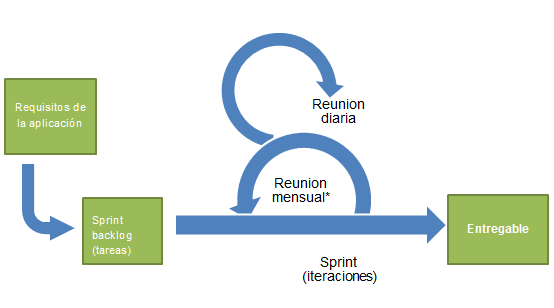
\includegraphics[scale=0.5]{../img/anexos/scrum-overview-es}
	\caption{Metodología \textit{scrum}~\cite{SCRUMWIKI}.}\label{img:scrum-overview}
\end{figure}

\subsubsection{\textit{Sprints}}
Los \textit{sprints} son periodos breves de \textbf{tiempo fijo} en el que el equipo trabaja para completar una cantidad de trabajo pre-establecida. Si bien muchas guías asocian los \textit{sprints} a la metodología ágil, asociando la metodología ágil y la metodología seguida en \textit{scrum} como si fueran lo mismo, cuando no lo son. La metodología ágil constituye una serie de principios, y la metodología \textit{scrum} es un marco de trabajo con la única finalidad de conseguir resultados.

A pesar de las similitudes los \textit{sprints} poseen un objetivo subyacente, entregar con frecuencia \textit{software} de trabajo.

\subsubsection{\textit{Sprint meetings}}
Dentro de la metodología \textit{scrum} existen diferentes reuniones que favorecen la agilidad del proyecto y que todo el mundo sepa lo que tiene que hacer en cada momento.
\begin{itemize}
\item \textbf{\textit{Sprint planning meeting.}} Esta reunión puede tener una duración de hasta de un día completo de trabajo. En ella deben de estar presentes todas las partes del proyecto, \textit{i.e.} el \textit{Scrum Master}, el equipo de desarrollo, y el \textit{product owner}. Poseen dos partes, en la primera de ellas se define el \textit{product backlog}, requerimientos del proyecto y se definen los objetivos para el \textit{sprint} que comienza, \textit{i.e.} lo que se espera ``construir'' o completar en el \textit{sprint}. En la segunda parte de la reunión se trabaja en el \textit{sprint backlog}, las tareas que se van a seguir en el \textit{sprint} para completar el objetivo de éste.
\item \textbf{\textit{Daily meeting.}} Debido a que los requerimientos del proyecto no se pueden variar durante la vida de un \textit{sprint}, existen las reuniones diarias que son organizadas por el \textit{Scrum Master} en las que se comenta el trabajo del día previo, lo que se espera de ese día y qué está retrasando o impidiendo a un individuo el proseguir con sus tareas, esta reunión no debe tener una duración de más de quince minutos y se debe realizar ``de pie''. No es una reunión para ver quién retrasa el proyecto sino para ayudar a quién lo necesite entre todos los miembros del equipo y permitir esa agilidad.
\item \textbf{\textit{Sprint review meeting.}} Reunión fijada al final de cada \textit{sprint} en la cual se hace una puesta en conocimiento de lo que se ha realizado en ese \textit{sprint}, siempre que se pueda se hará una demostración funcional en lugar de una presentación al \textit{product owner}. Esta reunión tiene un carácter informal.
\end{itemize}
 
\subsubsection{Artifacts}
Uno de los componentes más importantes de cara a la metodología \textit{scrum} son los artefactos, o \textit{artifacts} por su nombre en inglés. Éstos incluyen el \textit{product backlog}, el \textit{sprint backlog} y los \textit{burn down charts}.
\begin{itemize}
\item \textbf{\textit{Product backlog.}} Lista de trabajo ordenada por las prioridades para el equipo de desarrollo. Es generada a partir de las reuniones de planificación de los \textit{sprints}, contiene los requisitos. Se encuentra actualizado y clasificado en función de la periodicidad asignada a las tareas, pudiendo ser de corto o largo plazo. Aquellas tareas que se deban resolver a corto plazo deberán estar perfectaemnte descritas antes de asignarlas esta periodicidad, implicnddo que se han diseñado las historias de usuario completas así como el equipo de desarrollo ha establecido las estimaciones correspondientes. Los elementos a largo plazo pueden ser abstractos u opacos, conviene que estén estimados en la medida de lo posible para poder tener en cuenta el tiempo que llevará desarrollarla.

Los propietarios del producto dictan la prioridad de los elementos de trabajo en el \textit{product backlog}, mientras que el equipo de desarrollo dicta la velocidad a la que se trabaja en \textit{backlog}~\cite{danradigan2021}.

La estimación es una parte muy importante ya que es lo que permitirá al equipo de desarrollo mantener el ánimo y el trabajo al ritmo deseado. La estimación es realizada en la \textit{sprint planning meeting}, en la que se estima para cada tarea/producto del \textit{product backlog}. No se busca tener un resultado exacto del tiempo que va a llevar al equipo completar esa tarea, sino es una previsión. Para realizar correctamente la estimación se debe tener en cuenta el tamaño y la categoría de la tarea, los puntos de historia que se le van a asignar, así como el número de horas y días que van a ser necesarias para completar la tarea. 

\item \textbf{\textit{Sprint backlog.}} Lista de tareas extraídas del \textit{product backlog} que se han acordado desarrollarse a lo largo de un \textit{sprint}. Este \textit{backlog} es seleccionado por el propio equipo de desarrollo, para ello seleccionan una tarea del \textit{product backlog} y se divide en tareas de menor tamaño y abordables. Aquellas tareas de menor tamaño que el equipo no haya sido capaz de desarrollar previo a la finalización del \textit{sprint} quedarán almacenadas para próximos \textit{sprints} en el \textit{sprint backlog}.
\end{itemize}

\subsubsection{Actores, roles y responsabilidades}
Dentro de un equipo que sigue la metodología \textit{scrum} encontramos diferentes actores, como ya se ha comentado el equipo de desarrollo suele estar compuesto por entre cinco y diez personas, además del \textit{Scrum Master} y el \textit{Product Owner}~\cite{julioroche_2020}.
\begin{itemize}
\item \textbf{\textit{Product Owner.}} Encargado de optimizar y maximizar el valor del producto, es la persona encargada de gestionar las prioridades del \textit{product backlog}. Una de sus principales tareas es la de intermediario con los \textit{stakeholders}, partes interesadas, del proyecto; junto con recoger los requerimientos de los clientes. Es habitual que esta figura sea representante del negocio, con lo que aumenta su valor.

Para cada \textit{sprint} debe de marcar el objetivo de éste de manera clara y acordada con el equipo de desarrollo, lo cual hará que el producto vaya incrementando constantemente su valor. Para que todo fluya como debe, esta figura tiene que tener el ``poder'' de tomar decisiones que afecten al producto.

\item \textbf{\textit{Scrum Master.}} Figura con dos responsabilidades, gestionar el proceso \textit{scrum} y ayudar a eliminar impedimentos que puedan afectar a la entrega del producto.
\begin{enumerate}
\item Gestionar el proceso \textit{scrum}. Su función es asegurarse de que el proceso se lleva a cabo correctamente, facilitando la ejecución de éste y sus mecánicas. Consiguiendo que la metodología sea una fuente de generación de valor.
\item Eliminar impedimentos. Eliminar los problemas que vayan surgiendo a lo largo de los \textit{sprints} con el fin de mantener el ritmo de trabajo dentro de los equipos de desarrollo para poder entregar valor, manteniendo la integridad de la metodología.
\end{enumerate}
\item \textbf{Equipo de desarrollo.} Formado por entre cinco y diez personas encargados del desarrollo del producto, organizados de forma autónoma para conseguir entregar las tareas del \textit{product backlog} asignadas al \textit{sprint} correspondiente. Para que funcione correctamente la metodología todos los integrantes deben de conocer su rol dentro del equipo, internamente se pueden gestionar como el equipo considere, pero de cara ``hacia fuera'' son un equipo con una responsabilidad.
\end{itemize}
\newpage
\subsection{Planificación por \textit{sprints}}
La organización temporal del proyecto se ha organizado siguiendo los estándares de la metodología \textit{scrum}, \textit{i.e.} usando \textit{sprints}. 

Inicialmente la \textit{sprint planning meeting} es realizada cada dos semanas, debido a una falta de costumbre de trabajo con esta metodología se combina junto con la \textit{sprint review meeting}, de forma que en una sola reunión se comenta tanto lo que se ha hecho como lo que está por realizarse en el siguiente \textit{sprint}.

La velocidad de desarrollo del proyecto es una incógnita, debido a la no existencia de referencias previas del equipo de desarrollo del proyecto, en proyectos de ésta índole. Por lo tanto, la duración de los \textit{sprints} puede que se vea ajustada a lo largo de la vida del proyecto.

No se utilizan \textit{daily meetings} puesto que a pesar de que se invierte una media de tres a cinco horas diarias en el desarrollo, no es considerada necesaria. Si bien en caso de problemas se acuerda una reunión para el día siguiente con el fin de mantener la agilidad y no retrasar el proyecto.

\subsubsection{\textit{Sprint} 0: \textit{Lights out and away we go!} }
El \textit{sprint} con el que comienza el desarrollo de este proyecto no ha seguido la metodología \textit{scrum}, puesto que se formuló desde un punto de vista de toma de contacto inicial con el trabajo de investigación y todo lo que ello conlleva.

Los objetivos definidos han sido:
\begin{enumerate}
\item Lectura de \textit{papers} relacionados con el ámbito de la inteligencia artificial. En concreto \textit{SSL density peaks}~\cite{wu2018self}, \textit{Co-Training}~\cite{blum1998combining}, \textit{Tri-Training}~\cite{zhou2005tri} y \textit{Democratic Co-Learning}~\cite{zhou2004democratic}.
\end{enumerate}

El tiempo empleado en la lectura y asimilación de estos conceptos ha sido de catorce horas, es la primera vez que se leen \textit{papers} o artículos científicos completos procurando asimilar todos los conceptos de éstos. Se ha desarrollado entre el veintisiete de octubre y el cinco de noviembre, de dos mil veintiuno. 

\subsubsection{\textit{Sprint} 1: Chad}
\begin{itemize}
\item \textbf{\textit{Planning meeting}}\\
Objetivos del primer \textit{sprint}:
\begin{enumerate}
\item Lectura del API de \textit{scikit-learn}. Comprensión del funcionamiento de los transformadores y estimadores enfocado desde el punto de su programación.
\item Lectura de los \textit{papers On issues instance selection}~\cite{liu2002issues}, \textit{Comparison of instances seletion algorithms I. algorithms survey}~\cite{jankowski2004comparison} y \textit{Comparison of instance selection algorithms II. Results and comments}~\cite{grochowski2004comparison}.
\item Implementación de las técnicas de reducción del conjunto de entrenamiento, basados en $k$-NN.
\end{enumerate}

\item \textbf{Marcas temporales}\\
El \textit{sprint} se desarrolla entre 08/11/2021 y 19/11/2021. Han sido dedicadas al desarrollo del proyecto treinta horas.

\item \textbf{\textit{Burndown chart}}\\
\begin{figure}
\begin{center}
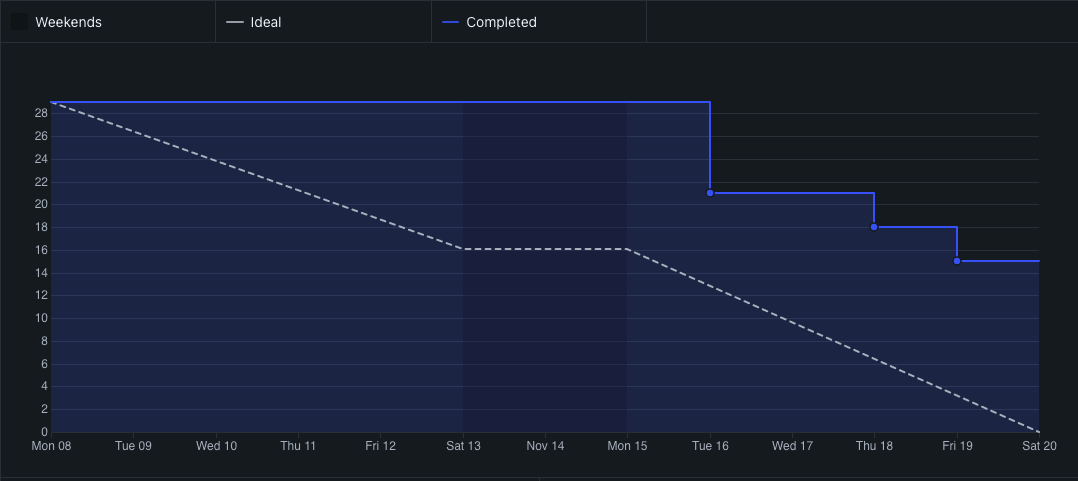
\includegraphics[width=\textwidth]{../img/anexos/sprints/BD-Sprint1}
\caption{\textit{Burndown Chart Sprint 1.}}\label{fig:BD-Sprint1}
\end{center}
\end{figure}
Durante este \textit{sprint} el trabajo inicial comenzó ligeramente retrasado, motivos en el apartado \textit{sprint review meeting}, por lo tanto podemos observar en la Figura ~\ref{fig:BD-Sprint1} como el trabajo completado dista del ideal o proyectado para este \textit{sprint}.

En el \textit{sprint backlog} habían sido incluidos todos los algoritmos a programar, es por ello que indica que se ha completado aproximadamente la mitad del trabajo.

\item \textbf{\textit{Sprint review meeting}}\\
El trabajo en este primer \textit{sprint} ha salido adelante correctamente. Al ser el primer \textit{sprint} ha habido un pequeño error de configuración del repositorio junto con la herramienta ZenHub, de ahí que en el \textit{burndown chart} de esta semana, Figura ~\ref{fig:BD-Sprint1}, aparezca como que la primera semana del \textit{sprint} no ha habido trabajo completado.

La adaptación a la metodología ágil ha resultado un poco compleja.
\end{itemize}

\subsubsection{\textit{Sprint} 2: Holleyman}
\begin{itemize}
\item \textbf{\textit{Planning meeting}}\\
Objetivos del segundo \textit{sprint}:
\begin{enumerate}
\item Finalizar implementación de los algoritmos basados en técnicas de reducción del conjunto de entrenamiento.
\item Añadir la documentación correspondiente a los algoritmos implementados.
\item Comprobar el rendimiento de los algoritmos implementados respecto a los resultados de una ejecución similar con el software \textit{Weka}.
\end{enumerate}
El \textit{sprint} se desarrolla entre el veintidós de noviembre y el tres de diciembre de dos mil veintiuno. Han sido dedicadas al desarrollo del proyecto treinta y ocho horas.

\item \textbf{Marcas temporales}\\
El \textit{sprint} se desarrolla entre 20/11/2021 y 04/12/2021.

\item \textbf{\textit{Burndown chart}}\\
\begin{figure}
\begin{center}
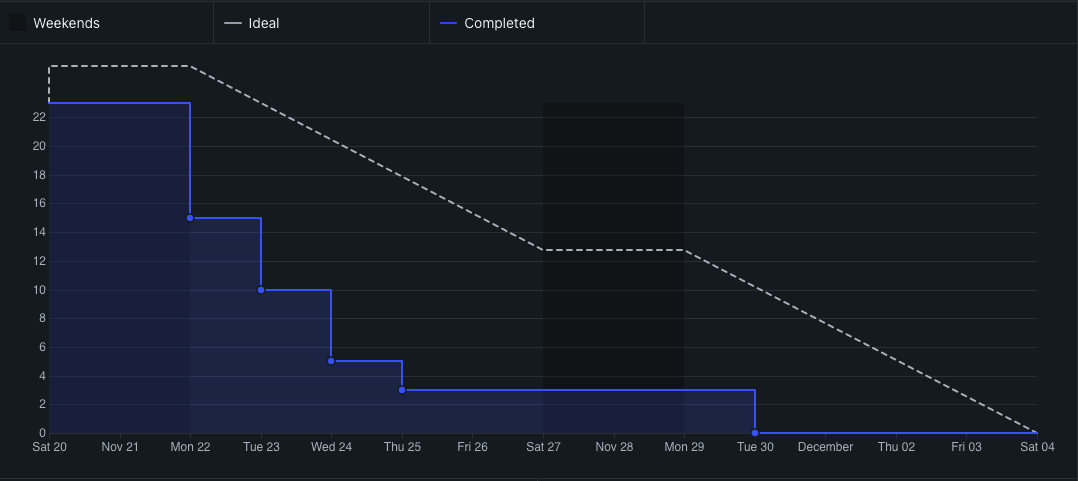
\includegraphics[width=\textwidth]{../img/anexos/sprints/BD-Sprint2}
\caption{\textit{Burndown Chart Sprint 2.}}\label{fig:BD-Sprint2}
\end{center}
\end{figure}
El trabajo realizado a lo largo de este \textit{sprint} ya ha sido adecuado a la metodología \textit{scrum}, obteniendo un \textit{burndown chart}, Figura ~\ref{fig:BD-Sprint2}, con más sentido que la que se había obtenido en el \textit{Sprint } 1. 

El equipo de desarrollo se sigue habituando poco a poco a la metodología de trabajo y en este \textit{sprint} se ha trabajo por debajo del <<ideal>> para el proyecto. 

\item \textbf{\textit{Sprint review meeting}}\\
A lo largo de este \textit{sprint} se descubrió un problema en la forma de identificar los $k$-NN en el algoritmo \textit{Condensed Nearest Neighbor, CNN}~\cite{hart1968condensed}, retrasando el trabajo cuatro horas, entre identificación y re-programación. Este error se descubrió mientras se investigaba otro error, en este caso el algoritmo \textit{Iterative Case Filtering, ICF}~\cite{brighton2002advances} terminaba en error buscando los k-NN de las últimas instancias.

La implementación de los algoritmos \textit{Reduced Nearest Neighbor, RNN}~\cite{gates1972reduced} y \textit{Modified Selective Subset, MSS}~\cite{barandela2005decision} ha sido relativamente asequible una vez se comprendía el algoritmo en cuestión así como su funcionamiento (entradas, procesado, salidas...).
\end{itemize}

\subsubsection{\textit{Sprint} 3: Manion}
\begin{itemize}
\item \textbf{\textit{Planning meeting}}\\
Objetivos del tercer \textit{sprint}:
\begin{enumerate}
\item Comenzar la documentación del proyecto.
\begin{itemize}
\item Comenzar la memoria por el marco teórico.
\item Comenzar los anexos por la planificación temporal.
\end{itemize} 
Se va a realizar en \LaTeX.
\item Aprender lo básico de \LaTeX{} lo más rápido posible para poder trabajar con él.
\item Buscar la precisión de los algoritmos implementados con conjuntos etiquetados de $[1\%, 5\%, 10\%, 20\%, 40\%, 60\%, 80\%, 100\%]$ del conjunto total. En búsqueda de las asíntotas donde ya no mejora la clasificación.
\item Validación de los algoritmos de selección de instancias con \texttt{Weka} y \texttt{KNN}.
\end{enumerate}

\item \textbf{Marcas temporales}\\
El \textit{sprint} se desarrolla entre el 06/12/2021 y el 17/12/2021. Han sido dedicadas al desarrollo del proyecto 45 horas.

\item \textbf{\textit{Burndown chart}}\\
El trabajo realizado en este tercer \textit{sprint} ha sido realizado a un ritmo constante y con una dedicación en número de horas un poco mayor a los anteriores, como se puede ver en el \textit{Burndown report}, ver figura~~\ref{fig:BD-Sprint3}, el número de \textit{story points} de este \textit{sprint} era de 39 y a pesar de que algunas tareas llevaron más tiempo del inicialmente planificado, otras resultaron ser totalmente lo contrario, mucho más rápidas de realizar.
\begin{figure}
\begin{center}
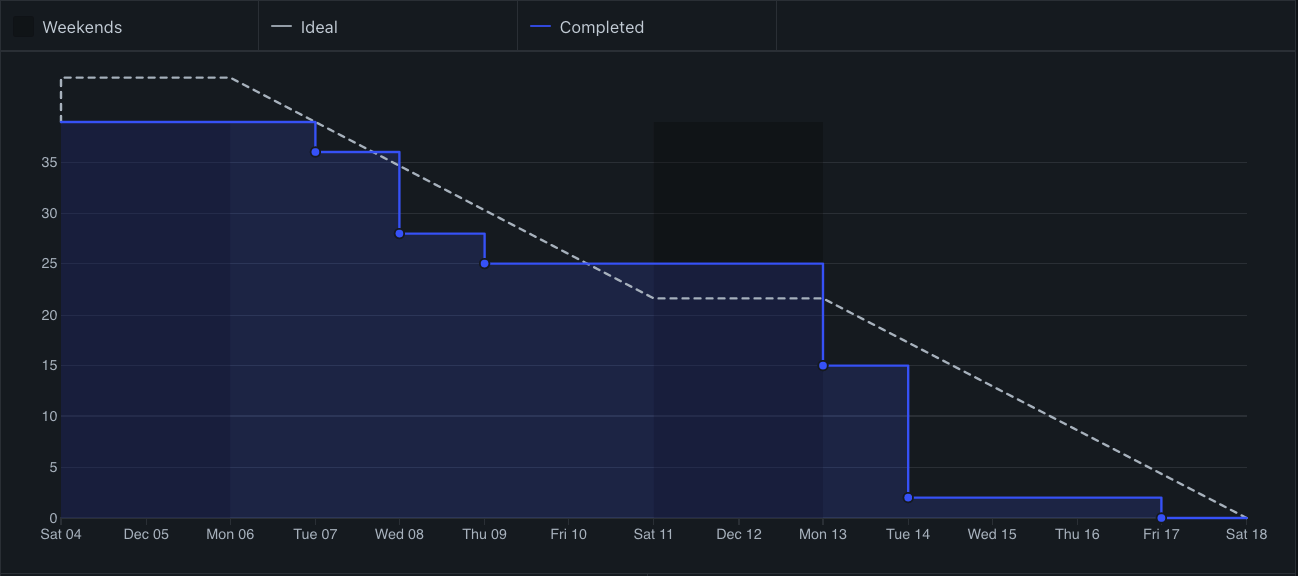
\includegraphics[width=\textwidth]{../img/anexos/sprints/BD-Sprint3}
\caption{\textit{Burndown Chart Sprint 3.}}\label{fig:BD-Sprint3}
\end{center}
\end{figure}
\item \textbf{\textit{Sprint review meeting}}\\
Este \textit{sprint} ha sido un poco más grande en cuanto a horas de trabajo invertidas ya que el tiempo del equipo de desarrollo así lo ha permitido. A su vez se han detectado \textit{bugs} en la codificación de algoritmos como ICF (se arreglará en el siguiente \textit{sprint}) el cual después de comparar sus resultados contra los expresados por \textit{Weka} con 9 conjuntos de datos no considerados como de juguete, la codificación del proyecto obtiene soluciones 20\% inferiores; el resto de los algoritmos implementados están en el rango de $\pm2\%$. A su vez también se han descubierto limitaciones de otros algoritmos como es el caso de ENN cuando tiene pocas muestras y un número elevado de clases diferentes.

Se ha proseguido con la redacción de la memoria del trabajo, finalizando la primera parte de conceptos teóricos y comenzando la explicación teórica de los algoritmos que
\end{itemize}

\subsubsection{\textit{Sprint} 4: The Seven}
\begin{itemize}
\item \textbf{\textit{Planning meeting}}\\
Objetivos del cuarto \textit{sprint}
\begin{enumerate}
\item Revisar y corregir la codificación del algoritmo \textit{Iterative Case Filtering}, \textit{ICF}.
\item Formatear las métricas de rendimiento recogidas durante el \textit{sprint} anterior.
\end{enumerate}

\item \textbf{Marcas temporales}\\
El \textit{sprint} se desarrolla entre el 18/12/2021 y el 23/12/2021. Han sido dedicadas al desarrollo del proyecto 21 horas. Este \textit{sprint} posee una duración más corta con el fin de ajustar las reuniones a las festividades propias de la Navidad.

\item \textbf{\textit{Burndown chart}}\\
En el \textit{Burndown report} asociado a este \textit{sprint}, ver figura~~\ref{fig:BD-Sprint4}, se aprecia como el trabajo ha sido finalizado  en unas marcas temporales muy por delante de lo <<ideal>>. Esto se debe a que el equipo de desarrolló comenzó a realizar el trabajo el sábado 18 de diciembre, en lugar de esperar al lunes 20, bajo la presunción de que el trabajo asignado iba a ser mayor.
\begin{figure}
\begin{center}
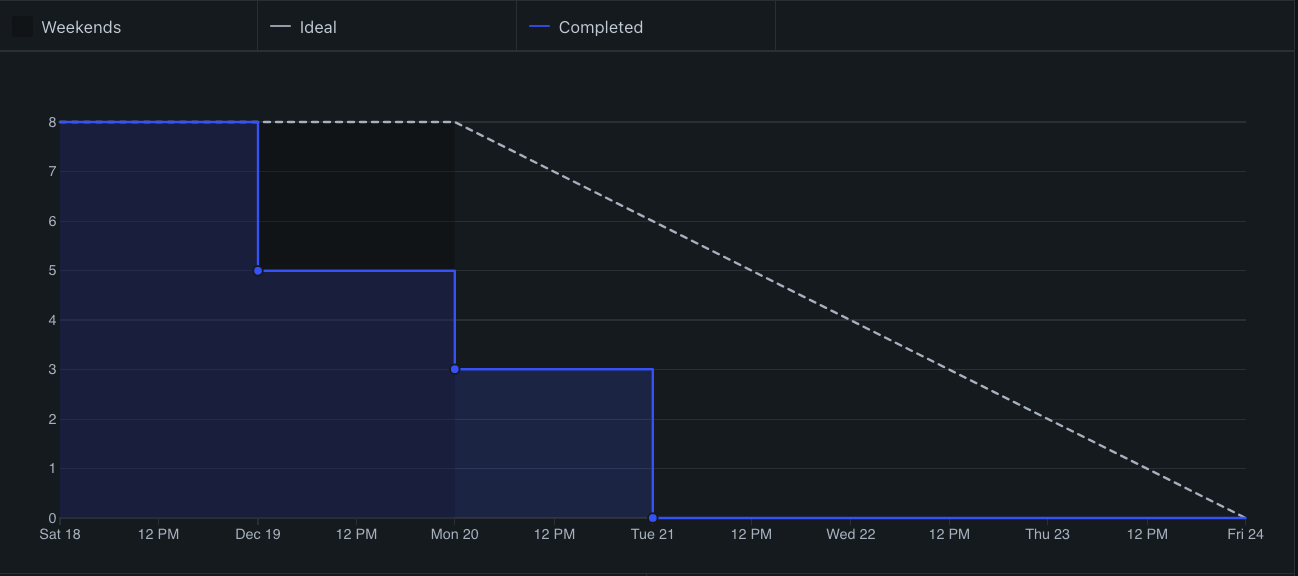
\includegraphics[width=\textwidth]{../img/anexos/sprints/BD-Sprint4}
\caption{\textit{Burndown Chart Sprint 4.}}\label{fig:BD-Sprint4}
\end{center}
\end{figure}

\item \textbf{\textit{Sprint review meeting}}\\
Ha pesar de la corta duración del \textit{sprint} para poder organizar el siguiente \textit{sprint} antes de las festividades navideñas, el trabajo realizado ha sido correcto e importante, debido a que para poder seguir trabajando en otros algoritmos de selección de instancias o de aprendizaje semi-supervisado, lo anterior debe de quedar correctamente hecho. Es por ello, que prácticamente se le ha dedicado un \textit{sprint} entero a arreglar el algoritmo \textit{Iterative Case Filtering, ICF}, ya que con él y a falta de implementar DROP3, ya tendríamos todos los algoritmos de selección de instancias correctamente implementados.
\end{itemize}
\vfill
\subsubsection{\textit{Sprint} 5: Murph}
\begin{itemize}
\item \textbf{\textit{Planning meeting}}\\
Objetivos del quinto \textit{sprint}:
\begin{enumerate}
\item Codificación de los algoritmos de aprendizaje semi-supervisado: Co-Training~\cite{blum1998combining}, Tri-Training~\cite{zhou2005tri}, Democratic Co-Learning~\cite{zhou2004democratic}. Y el algoritmo de selección de instancias DROP3~\cite{wilson2000reduction}.
\item Implementar los algoritmos anteriores como clases para poder ser utilizados con métodos \textit{fit} y \textit{predict}.
\item Escribir la documentación de la memoria referente a los anteriores algoritmos.
\item Escribir la planificación temporal relativa a los \textit{sprints} 4 y 5.
\item Añadir leyenda a la figuras generadas con \textit{self-training} en función de un \% de datos etiquetados.
\end{enumerate}
Se espera que sea un \textit{sprint} muy productivo debido a las fechas en las que se realiza y la mayor disponibilidad del equipo de desarrollo.

\item \textbf{Marcas temporales}\\
Este \textit{sprint} se desarrolla entre el 24/12/2021 y el 10/01/2022. Tiene una duración igual a las festividades navideñas.
\item \textbf{\textit{Burndown chart}}\\
\begin{figure}
\begin{center}
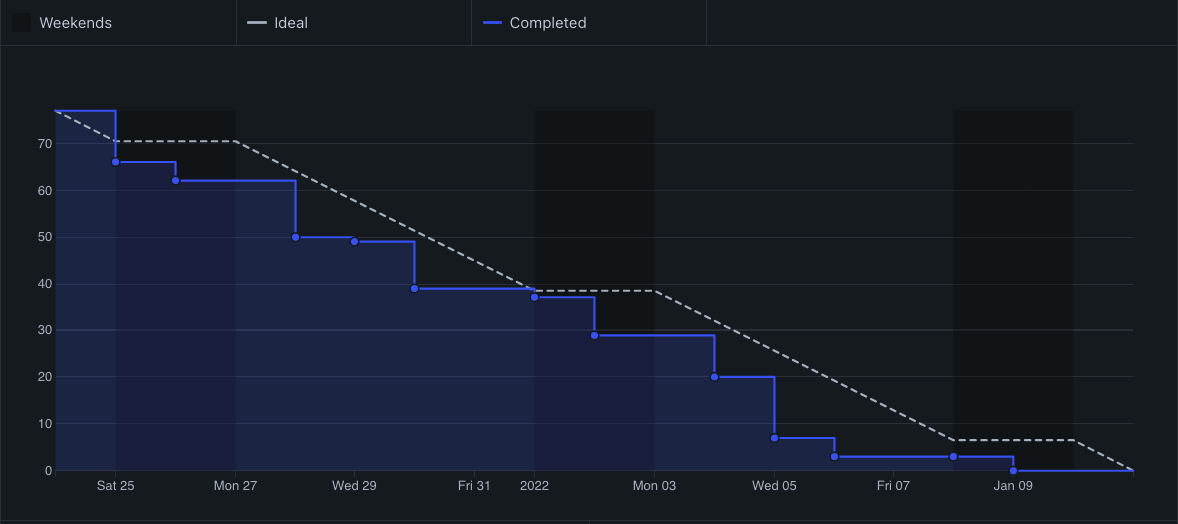
\includegraphics[width=\textwidth]{../img/anexos/sprints/BD-Sprint5}
\caption{\textit{Burndown Chart Sprint 5.}}\label{fig:BD-Sprint5}
\end{center}
\end{figure}
En este \textit{sprint}, y como vemos en la figura~\ref{fig:BD-Sprint5}, referente al correspondiente \textit{Burndown report}; se ha realizado una gran cantidad de trabajo, habiendo siendo completados 77 puntos de historia, una cantidad muy superior a anteriores \textit{sprints}, esto es debido en gran parte a las fechas en las que nos encontramos, ya que el número de horas que se han podido invertir en el desarrollo del proyecto ha sido muy superior a lo que venían siendo habituales. En total han sido utilizadas cerca de 110 horas de trabajo, siendo repartidas en los 17 días que ha durado el \textit{sprint} y con una media de horas de trabajo de 6.5 horas diarias. 

\item \textbf{\textit{Sprint review meeting}}\\
Todo el trabajo que se ha realizado en este \textit{sprint} podría haber sido realizado seguramente en tres cuartas partes del tiempo real invertido, pero debido al tiempo de lectura de los artículos de donde se extraían los algoritmos, así como su correcta comprensión, codificación y posterior resolución de problemas asociados a \textit{bugs} que se van descubriendo <<sobre la marcha>>, ha sido un \textit{sprint} largo y en algunos momentos agotador. 

A falta de realizar las correspondientes pruebas de validación de los algoritmos implementados, para comprobar que son correctas las implementaciones, ya se encontrarían finalizados todos los algoritmos de selección de instancias.

\end{itemize}
\subsubsection{\textit{Sprint} 6: Bert}
\begin{itemize}
\item \textbf{\textit{Planning meeting}}\\
Objetivos del sexto \textit{sprint}:
\begin{enumerate}
\item Verificación de la correcta implementación del algoritmo de selección de instancias DROP3. Se realizará como se ha venido trabajando anteriormente, contra los resultados propuestos para la misma parametrización, por Weka.
\item Verificación de la correcta implementación de los algoritmos de aprendizaje semi-supervisado: \textit{Co-Training}, \textit{Tri-Training} y \textit{Democratic Co-Learning}.
\item Comenzar a escribir las secciones de <<Técnicas y herramientas>> y <<Trabajos relacionados>>.
\end{enumerate}

\item \textbf{Marcas temporales}\\
Este es un \textit{sprint} relativamente corto, puesto que es de verificación de que el trabajo realizado hasta el momento es correcto, antes de pasar a otro <<bloque>> de trabajo. Comienza el martes 11/01/2022, y finaliza el lunes 17/01/2022.

\item \textbf{\textit{Burndown chart}}\\
\begin{figure}
\begin{center}
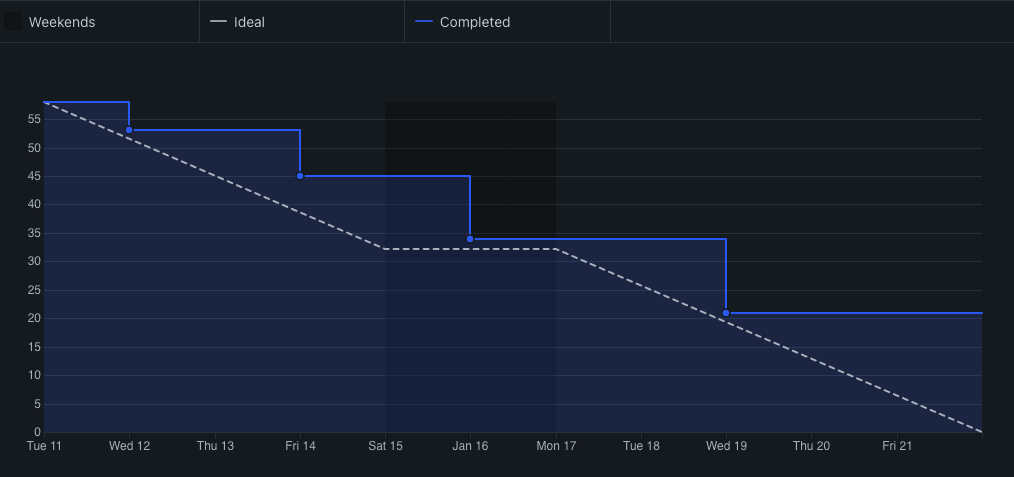
\includegraphics[width=\textwidth]{../img/anexos/sprints/BD-Sprint6}
\caption{\textit{Burndown Chart Sprint 6.}}\label{fig:BD-Sprint6}
\end{center}
\end{figure}
Tal y como se aprecia en la Figura~\ref{fig:BD-Sprint6} referente al sexto \textit{sprint}, el ritmo de trabajo ha sido constante a lo largo de la primera semana, torciéndose al final del \textit{sprint} debido a la complejidad sobrellevada de aprender la biblioteca \textit{Flask} y sus dependencias. Es por ello que dos \textit{issues} se cerraron un día más tarde de la planificación.
El número de horas aproximado que se han invertido han sido de 50h, permitido en gran medida con que todavía no hay clases del segundo cuatrimestre.

\item \textbf{\textit{Sprint review meeting}}\\
El trabajo realizado en este \textit{sprint} ha ido de acuerdo a lo que se comentó en la anterior reunión. Si bien ha sido un \textit{sprint} más enfocado a <<cerrar>> una parte de trabajo que se llevaba realizada para poder comenzar con el mejor pie posible la segunda etapa.

Un punto de inflexión realizado en este \textit{sprint} ha sido la refactorización de gran parte del repositorio, dejándolo en un formato de paquetes.
\end{itemize}

\subsubsection{\textit{Sprint} 7: Felix The Cat}
\begin{itemize}
\item \textbf{\textit{Planning meeting}}\\
Objetivos del séptimo \textit{sprint}:
\begin{enumerate}
\item Modificar el algoritmo ENN para poder utilizarlo con Semi-Supervisado según el método de borrado de instancias.
\item Preparar \textit{scripts} para la experimentación y posterior visualización de hipótesis.
\item Modificar la memoria en función de los comentarios de Alvar.
\item Añadir a los trabajos relacionados UBUMLaaS. Aunque es parte del propio Trabajo de Fin de Grado, no deja de ser una herramienta de MLaaS.
\item Añadir \textit{Self Training} a UBUMLaaS.
\end{enumerate}

\item \textbf{Marcas temporales}\\
Este \textit{sprint} se desarrolla entre el 25/01/2022 y el 02/02/2022. Es un \textit{sprint} muy rápido de preparación para poder comenzar con la parte de UBUMLaaS.

\item \textbf{\textit{Burndown chart}}\\
\begin{figure}
\begin{center}
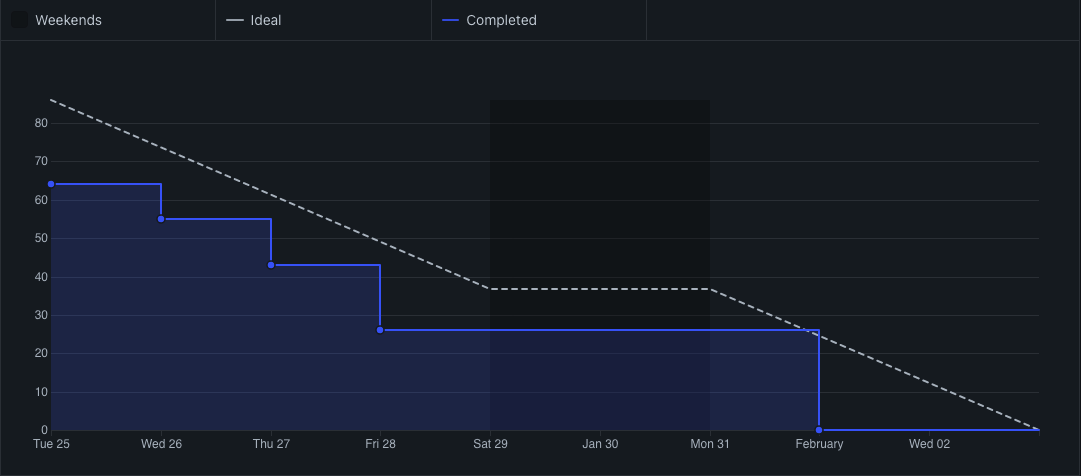
\includegraphics[width=\textwidth]{../img/anexos/sprints/BD-Sprint7}
\caption{\textit{Burndown Chart Sprint 7.}}\label{fig:BD-Sprint7}
\end{center}
\end{figure}
El \textit{Burndown} de este \textit{sprint} representa un ritmo de trabajo <<adelantado>> a la velocidad óptima, esto se debe a que como en el \textit{sprint} anterior no se cerraron todas las \textit{issues} previa la finalización del mismo, pero sí fueron cerradas previo el inicio de este nuevo \textit{sprint}, el gráfico queda por debajo siempre. El número de horas invertido ha rondado las 35h. Un \textit{sprint} de menor tamaño.

\item \textbf{\textit{Sprint review meeting}}\\
Este \textit{sprint} si bien es como el anterior muy corto, y se ajusta a la temporarización del proyecto, ha tenido una carga de trabajo un poco más alta de lo esperado, esto se debe a que la integración de nuevos algoritmos a UBUMLaaS parecía en un primer momento muy directo, pero se han requerido hacer modificaciones con las que no se contaba en un primer momento.

\end{itemize}

\subsubsection{\textit{Sprint} 8: Jason}
\begin{itemize}
\item \textbf{\textit{Planning meeting}}\\
Objetivos del octavo \textit{sprint}:
\begin{enumerate}
\item Crear una nueva selección en <<Nuevo Experimento>> en UBUMLaaS para los algoritmos de aprendizaje Semi-Supervisado.
\item Integrar los algoritmos implementados de Semi-Supervisado en la plataforma UBUMLaaS.
\item Comenzar a traducir parte de la interfaz como parte de un trabajo paralelo. (Puede que la versión final soporte varios idiomas, decisión de diseño aún por tomar.)
\item Crear los rankings con Python de las experimentaciones realizadas, principalmente de 3-NN sin borrado.
\item Hacer un \textit{refactor} general al proyecto. Inicialmente tenía una estructura de carpetas, se desea una estructura de paquetes.
\item Hacer el proyecto accesible desde PIP\footnote{Sistema de gestión de paquetes utilizado para instalar y administrar paquetes de \textit{software} escritos en Python.}.
\end{enumerate}

\item \textbf{Marcas temporales}\\
Este \textit{sprint} se desarrolla entre el 03/02/2022 y el 08/02/2022. Nos encontramos ante otro \textit{sprint} ya con la nueva dinámica de trabajo, de duración aproximada a una semana.

\item \textbf{\textit{Burndown chart}}\\
\begin{figure}
\begin{center}
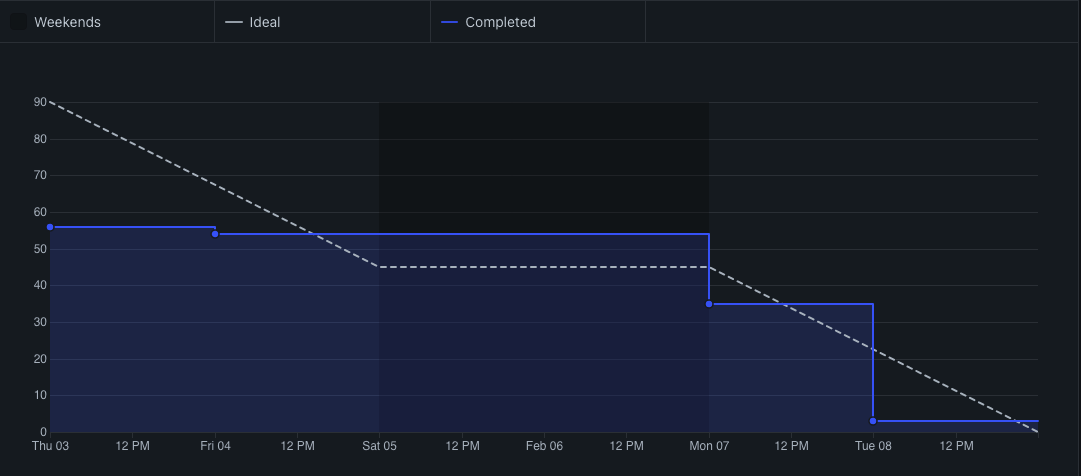
\includegraphics[width=\textwidth]{../img/anexos/sprints/BD-Sprint8}
\caption{\textit{Burndown Chart Sprint 8.}}\label{fig:BD-Sprint8}
\end{center}
\end{figure}
Tal y como se aprecia en la Figura~\ref{fig:BD-Sprint8} se aprecia que el ritmo de trabajo en este \textit{sprint} ha sido muy escalonado, el número de \textit{issues} no ha sido muy elevado, pero la complejidad de estas sí que lo ha sido, es por ello que se planificó 90 puntos de historia. Seguidamente podemos apreciar como entre el cuatro y el siete de febrero, coincidiendo con el fin de semana, no ha habido trabajo finalizado, se debe a unas mini-vacaciones que se tomó el equipo de desarrollo.

\item \textbf{\textit{Sprint review meeting}}\\
Con el \textit{sprint} finalizado se ha visto como lo que parecía una planificación para una o dos semanas, ha quedado resuelta dentro del propio \textit{sprint}. El equipo de desarrollo comienza a familiarizarse con el \textit{backend} de UBUMLaaS propiciando un desarrollo más eficaz de las tareas que se van encomiando.

Destacar que no se finalizan todas las tareas en tiempo, sino que se finaliza una en la noche del martes ocho, ya casi de madrugada, entrando técnicamente en el siguiente \textit{sprint}.

\end{itemize}

\subsubsection{\textit{Sprint} 9: Lumberjack 20}
\begin{itemize}
\item \textbf{\textit{Planning meeting}}\\
Objetivos del noveno \textit{sprint}:
\begin{enumerate}
\item Continuar con la traducción del \textit{frontend} en los <<tiempos muertos>>, aún no se ha decidido si finalmente pasará a producción o no.
\item Crear un nuevo conjunto de gráficas y relanzar experimentaciones con SVC como referencia. El método de eliminación de instancias con etiqueta conocida queda descartado, únicamente se trabajará para la experimentación con la aproximación que no las elimina.
\item Crear los nuevos rankings basados en la precisión. 
\item Comprobar la implementación de los algoritmos \textit{Co-Training}, \textit{Tri-Training} y \textit{Democratic Co-Learning} contra los implementados por Jose Luis Garrido Labrador (Investigador del grupo ADMIRABLE).
\item Añadir a UBUMLaaS los filtros implementados en los anteriores \textit{sprints}.
\end{enumerate}

\item \textbf{Marcas temporales}\\
Este \textit{sprint} se desarrolla entre el 09/02/2022 y el 16/02/2022.

\item \textbf{\textit{Burndown chart}}\\
\begin{figure}
\begin{center}
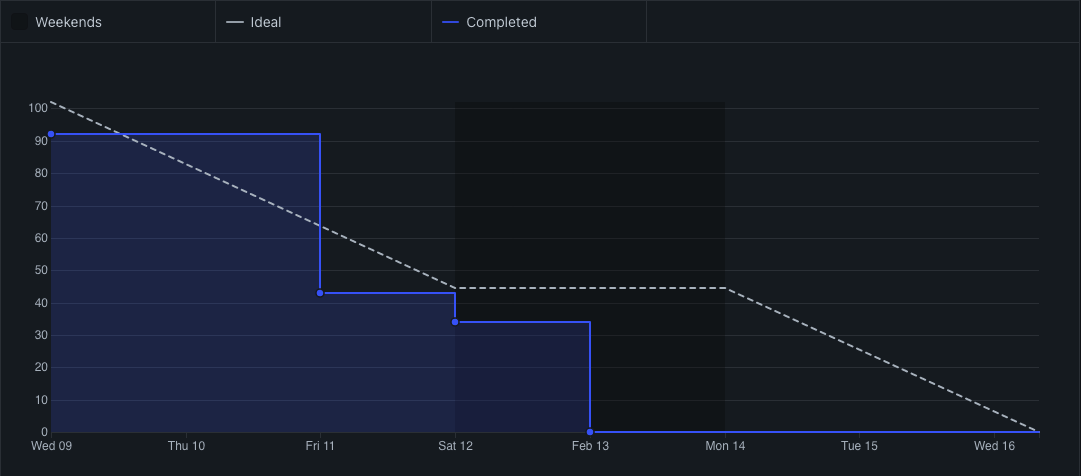
\includegraphics[width=\textwidth]{../img/anexos/sprints/BD-Sprint9}
\caption{\textit{Burndown Chart Sprint 9.}}\label{fig:BD-Sprint9}
\end{center}
\end{figure}
Este \textit{sprint} tiene una duración de una semana, tal y como se desea (aproximadamente) que sean a partir de febrero. A este \textit{sprint} se le asignó una gran carga en cuanto a puntos de historia se refiere con un total de 102, las horas invertidas por el equipo de desarrollo no han llegado a las 55, hay una desviación de los puntos de historia y las horas invertidas, se comentará más adelante.

Quedando el trabajo finalizado un par de días antes de la fecha de finalización del \textit{sprint}, dando al equipo de desarrollo tiempo para planear futuras tareas y aproximaciones a problemas conocidos.

\item \textbf{\textit{Sprint review meeting}}\\
En este \textit{sprint} se planificó <<tirando a lo alto>> en los puntos de historia, se debe a que se requería comprobar la implementación de los tres algoritmos de aprendizaje Semi-Supervisado, y en caso de que alguno (o todos) tuviera una implementación incorrecta, realizar los ajustes pertinentes para que fuera correcta. Debido a la experiencia del equipo de desarrollo un mes atrás con el filtro ICF, el cual tuvo que ser re-programado y revisado en más de una ocasión debido a su inconsistencia, se aventuró un futuro similar con éstos algoritmos ya que son más grandes y con una complejidad superior. La realidad en este caso superó las expectativas del equipo de desarrollo, cuando los tres algoritmos tuvieron una desviación menor al 1\% en comparación con los de Jose Luis. (En futuros \textit{sprints} se ha propuesto ser más críticos con la asignación de puntos de historia para no tener diferencias de este calibre).

Con todo y con ello, la implementación de los filtros en UBUMLaaS incurrió en múltiples modificaciones a la estructura base de la propia plataforma, pero con un resultado satisfactorio.

Los rankings creados no han convencido en estructura y formato, es por ello que en siguiente \textit{sprint} tendrán que ser repetidos.
\end{itemize}

\subsubsection{\textit{Sprint} 10: Jerry}
\begin{itemize}
\item \textbf{\textit{Planning meeting}}\\
Objetivos del décimo \textit{sprint}:
\begin{enumerate}
\item Rehacer las gráficas de rankings en la experimentación.
\item Comenzar con la parte de administración de UBUMLaaS.
\begin{enumerate}
\item Crear una nueva interfaz que de soporte a esta nueva funcionalidad que va a poseer la aplicación.
\item Integrar nuevos campos en el registro de usuarios, tales como su país de origen y el uso deseado que se le va a dar a aplicación.
\item Crear una interfaz de administración de usuarios (añadir usuarios, activarlos, hacerlos administradores o eliminarlos).
\item Crear una primera interfaz básica de \textit{dashboard analytics} del sistema.
\end{enumerate}
\end{enumerate}

\item \textbf{Marcas temporales}\\
Este \textit{sprint} se desarrolla entre el 16/02/2022 y el 21/02/2022.

\item \textbf{\textit{Burndown chart}}\\
\begin{figure}
\begin{center}
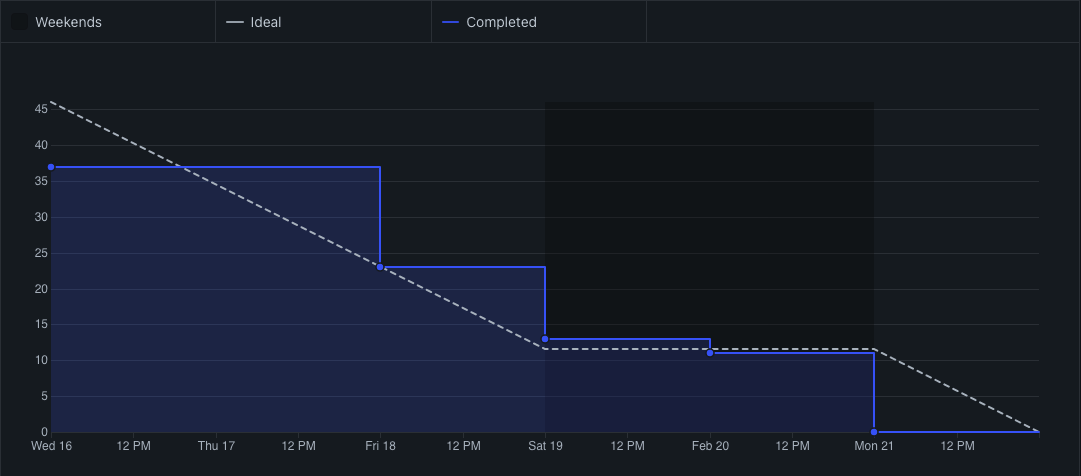
\includegraphics[width=\textwidth]{../img/anexos/sprints/BD-Sprint10}
\caption{\textit{Burndown Chart Sprint 10.}}\label{fig:BD-Sprint10}
\end{center}
\end{figure}
Este \textit{sprint} ha sido más ajustado el número de horas invertidas en el desarrollo de las tareas marcadas en comparación los puntos de historia. Se han marcado un total de 46 puntos de historia y se han invertido 35 horas de trabajo. Siguiendo un poco más la tónica de otros \textit{sprints}. En los primeros días, tal y como se aprecia en la Figura~\ref{fig:BD-Sprint10}, sí que hubo \textit{commits} pero no se cerraron tareas debido a que se trabajó en <<paralelo>> sobre varias \textit{issues} a la vez, ya que toda la parte de crear la interfaz de administración y las páginas que la iban a comenzar a formar parte de la misma, se encuentran fuertemente inter-relacionadas.

\item \textbf{\textit{Sprint review meeting}}\\
El trabajo realizado durante este \textit{sprint} ha sido más duro que el de \textit{sprints} anteriores. Esto se debe a la poca experiencia del equipo de desarrollo con aplicaciones que poseen un \textit{frontend}, el uso de JavaScript, jQuery, AJAX,\dots es algo que hasta la fecha no se había utilizado en gran medida y ahora es con lo que más se está trabajando, entonces ha requerido de un esfuerzo extra.

La parte de administración de UBUMLaaS ha sido creada con una base más moderna, sencilla y clara. Siguiendo el esquema de colores de la Universidad de Burgos. Es por ello que ahora mismo parecen dos aplicaciones diferentes, (la parte de administración en comparación con la parte de funcionalidad de MLaaS propiamente dicha).

Durante la realización del \textit{sprint} fueron surgiendo pequeños \textit{bugs} en la interfaz gráfica que se fueron solventando, todos ellos originados por descuidos (debido a la falta de experiencia) del propio equipo de desarrollo con el uso de las nuevas librarías.
\end{itemize}

\subsubsection{\textit{Sprint} 11: Nutts}
\begin{itemize}
\item \textbf{\textit{Planning meeting}}\\
Objetivos del undécimo \textit{sprint}:
\begin{enumerate}
\item Con~\cite{LI2019104895} se desea comprobar con 16 de los 18 conjuntos de datos utilizados en sus experimentos los resultados esperados para comprobar si merece la pena continuar la línea de investigación con el enfoque inicial.

\item Montar un servidor con Jenkins, se desea incorporar a UBUMLaaS y a la biblioteca $IS\_SSL$ dentro de CI/CD~\footnote{Método de distribución de aplicaciones a los clientes con una cierta frecuencia mediante el uso de la automatización en las etapas del desarrollo de aplicaciones. Se trata de una solución para los problemas que se pueden generar en la integración del código nuevo en producción.}
\item Añadir al \textit{dashboard analytics} gráficos de carta con el número de experimentos de cada tipo que se han ejecutado. Así como los tiempos de uso de cada algoritmo.
\item Crear una pantalla de carga para el \textit{dashboard} de forma que la recuperación de datos sea asíncrona.
\item Permitir al usuario añadir más datos personales dentro de su perfil (Institución,  redes sociales, \dots)
\item Realizar una nueva página de usuarios con la nueva distribución.
\item Permitir al usuario ver sus propias estadísticas de uso. 
\item Pantalla tipo \textit{dashboard} con el estado en directo del sistema.
\end{enumerate}

\item \textbf{Marcas temporales}\\
Este \textit{sprint} se desarrolla entre el 22/02/2022 y el 01/03/2022.

\item \textbf{\textit{Burndown chart}}\\
\begin{figure}
\begin{center}
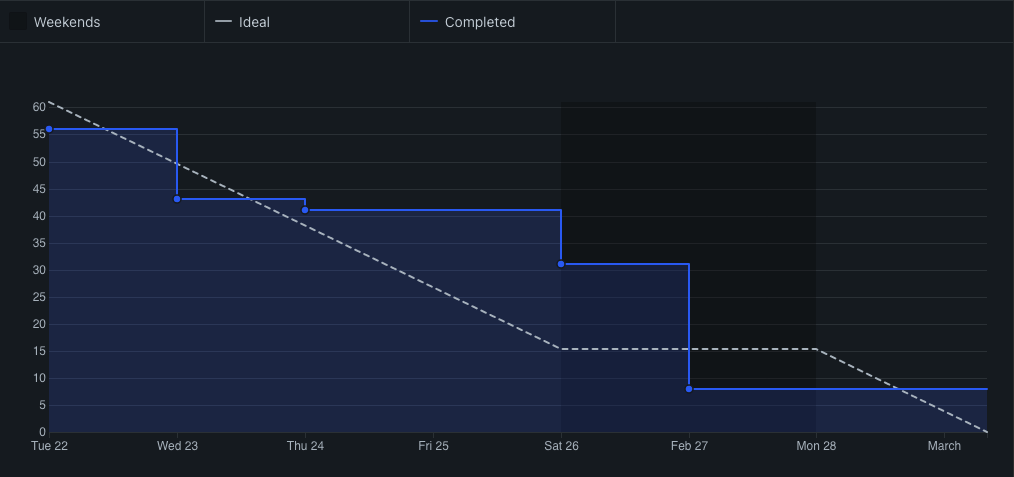
\includegraphics[width=\textwidth]{../img/anexos/sprints/BD-Sprint11}
\caption{\textit{Burndown Chart Sprint 11.}}\label{fig:BD-Sprint11}
\end{center}
\end{figure}
Con una duración de algo más de una semana, se han planificado un total de 58 puntos de historia para estos días. Las horas de trabajo han sido cercanas a las 45. La sensación del equipo de desarrollo después de haber finalizado el \textit{sprint} es de un trabajo a ritmo constante finalizando tarea tras tarea, esta sensación se puede comprobar como en efecto ha sido así en la Figura~\ref{fig:BD-Sprint11}.

\item \textbf{\textit{Sprint review meeting}}\\
En este \textit{sprint} no se han podido terminar todas las tareas, si bien en el servidor local en el que corre UBUMLaaS se ha podido desplegar Jenkins, el \textit{pipeline} para que funcione correctamente no se ha podido terminar. Igual se buscan otras alternativas que además den soporte a elementos como las \textit{badges} de GitHub y visualización de si pasan o no los tests en los propios \textit{commits}.

Las principales pantallas de administración van quedando mejor con cada \textit{sprint}, más retoques se las van haciendo y el equipo de desarrollo poco a poco comienza a sentirse más cómodo trabajando con lenguajes de marcas como es HTML, o de programación como JavaScript.

El número de horas invertidas en las que no se está programando como tal, sino que se requieren de aprendizaje previo a poder escribir código y hacer la tarea X que toque, sigue siendo alto en esta parte del proyecto.

\end{itemize}

\subsubsection{\textit{Sprint} 12: DVB}
\begin{itemize}
\item \textbf{\textit{Planning meeting}}\\
Objetivos del duodécimo \textit{sprint}:
\begin{enumerate}
\item Se ha decidido dejar <<en pausa>> la traducción de UBUMLaaS a idiomas como el castellano o el francés. No se descarta retomarlo en un futuro o que sean líneas de trabajo futuro.
\item Con la parte de administración ya más avanzada y con una cohesión mayor, se ha tomado la decisión de dar un <<lavado de cara>> a toda la aplicación, esto implica rehacer \textbf{todas} las páginas del \textit{frontend} con el fin de que se adapten a la nueva guía de estilo de la aplicación.
\item Realizar pequeños ajustes a ejes de gráficos.
\item Decidir e implementar una forma de toma de datos en tiempo real del sistema anfitrión para en posteriores \textit{sprints} visualizar esa información.
\item Implementación del algoritmo de aprendizaje Semi-Supervisado basado en picos de densidad, ver~\cite{WU2018180}.
\end{enumerate}

\item \textbf{Marcas temporales}\\
Este \textit{sprint} se desarrolla entre el 01/03/2022 y el 08/03/2022.

\item \textbf{\textit{Burndown chart}}\\
\begin{figure}
\begin{center}
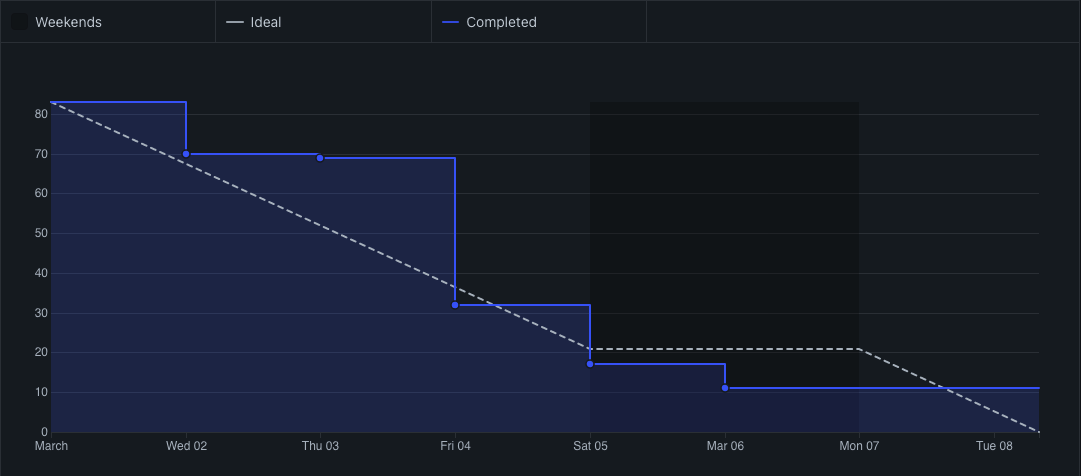
\includegraphics[width=\textwidth]{../img/anexos/sprints/BD-Sprint12}
\caption{\textit{Burndown Chart Sprint 12.}}\label{fig:BD-Sprint12}
\end{center}
\end{figure}
El trabajo realizado en este \textit{sprint} tal y como en la Figura~\ref{fig:BD-Sprint12} se aprecia, ha sido superior a los anteriores, con un total de 83 puntos de historia y cerca de 45 horas invertidas. En esta ocasión el trabajo ha vuelto ha ser planificado <<por lo alto>> debido a la suposición de complejidad de implementación del algoritmo de aprendizaje Semi-Supervisado. 

\item \textbf{\textit{Sprint review meeting}}\\
En este \textit{sprint} el equipo de desarrollo ha tenido la sensación que no <<llegaba>> a todo lo planificado, las reuniones llegan a un punto en el cuál se comenta trabajo, queda apuntado, y se intenta meter todo en tiempo y forma. Generando un cierto agobio en algunas situaciones que han impedido continuar con el trabajo al ritmo deseado.

En líneas generales se puede afirmar que el \textit{frontend} ha sido rehecho entero, se han reutilizado formatos o formularios existentes por facilidad de uso a todos aquellos usuarios que ya la conocieran, pero a nivel de código prácticamente es nueva. Con un estilo mucho más moderno, fino y elegante.

La integración de CI/CD finalmente ha quedado hecha con elementos \textit{cloud}, entre ellos se encuentran Travis-CI, Codebeat, SonarCloud y Codacy. Debido a que se ha rehecho toda la interfaz web de la aplicación, los tests existentes no pasan, es por ello que se tendrán que rehacer poco a poco, aunque no es uno de los elementos de mayor prioridad por el momento.

\end{itemize}

\subsubsection{\textit{Sprint} 13: Kutschbach}
\begin{itemize}
\item \textbf{\textit{Planning meeting}}\\
Objetivos del decimotercero \textit{sprint}:
\begin{enumerate}
\item Implementación del algoritmo de aprendizaje Semi-Supervisado basado en picos de densidad con filtrado, ver~\cite{LI2019104895}.
\item Mejora inicial de la calidad del código.
\item Panel \textit{dashboard} de visualización de estado del sistema en tiempo real.
\item Dar soporte a que el usuario pueda cambiar su foto de perfil.
\item Realizar algunas pruebas de estrés para detectar puntos de rotura de la interfaz.
\item Comenzar a escribir los Requisitos.
\item Comenzar a escribir dentro del Diseño, el diagrama de casos de uso.
\item Añadir a los aspectos relevantes los métodos que se están haciendo a sí como los cambios en la interfaz.
\item Revisar comentarios hechos por Alvar en la memoria.
\end{enumerate}

\item \textbf{Marcas temporales}\\
Este \textit{sprint} se desarrolla entre el 08/03/2022 y el 15/03/2022.

\item \textbf{\textit{Burndown chart}}\\
\begin{figure}
\begin{center}
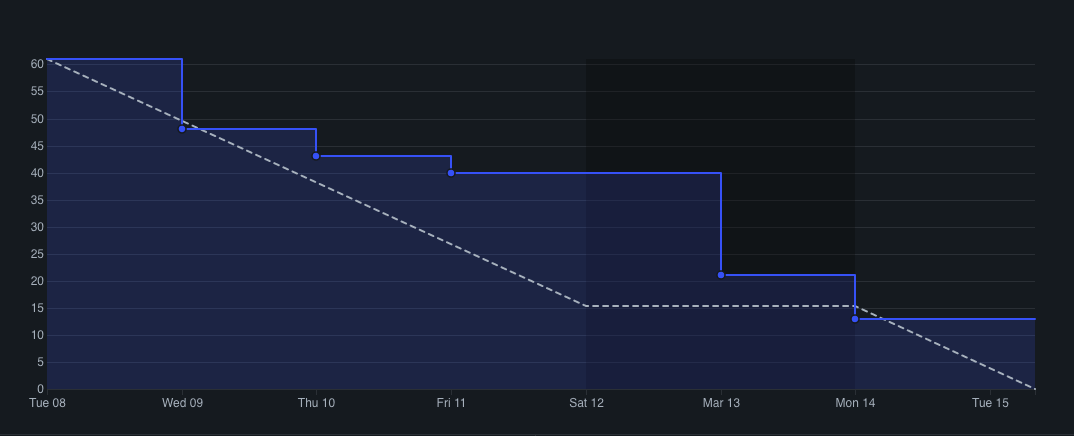
\includegraphics[width=\textwidth]{../img/anexos/sprints/BD-Sprint13}
\caption{\textit{Burndown Chart Sprint 13.}}\label{fig:BD-Sprint13}
\end{center}
\end{figure}
Tal y como se aprecia en la Figura~\ref{fig:BD-Sprint13}, en este \textit{sprint} el ritmo de trabajo ha sido muy constante, algunas tareas fueron asignadas con puntos de historia más bajos de lo que deberían de haber sido y así quedan reflejados en los días diez y once. El total de puntos de historia ha sido de 48 con un total de 30 horas invertidas.

\item \textbf{\textit{Sprint review meeting}}\\
El trabajo realizado en este \textit{sprint} ha sido satisfactorio a pesar de que no se han podido terminar todas las tareas abiertas a tiempo, esto ha sido debido a un pequeño bajón en la motivación del equipo de desarrollo junto con otras actividades de la vida universitaria. \\
En lo referido al proyecto, han surgido múltiples reconsideraciones del diseño de la interfaz según se iban recuperando datos y diseñando, por lo que el proceso de trabajo ha tenido un componente creativo en muchas ocasiones, no siendo el principal fuerte del equipo de desarrollo.
\end{itemize}

\subsubsection{\textit{Sprint} 14: T.U.P.}
\begin{itemize}
\item \textbf{\textit{Planning meeting}}\\
Objetivos del decimocuarto \textit{sprint}:
\begin{enumerate}
\item Ultimar detalles de los casos de uso.
\item Hacer diagramas de secuencia de <<Nuevo Experimento>>, <<Consultar Analíticas de Uso>> y <<Monitorización en tiempo real>>.
\item Realizar la experimentación con picos de densidad y ruido.
\item Implementación de los algoritmos LSSm y LSBo, ver~\cite{leyva2015three}.
\end{enumerate}

\item \textbf{Marcas temporales}\\
Este \textit{sprint} se desarrolla entre el 15/03/2022 y el 22/03/2022.

\item \textbf{\textit{Burndown chart}}\\
\begin{figure}
\begin{center}
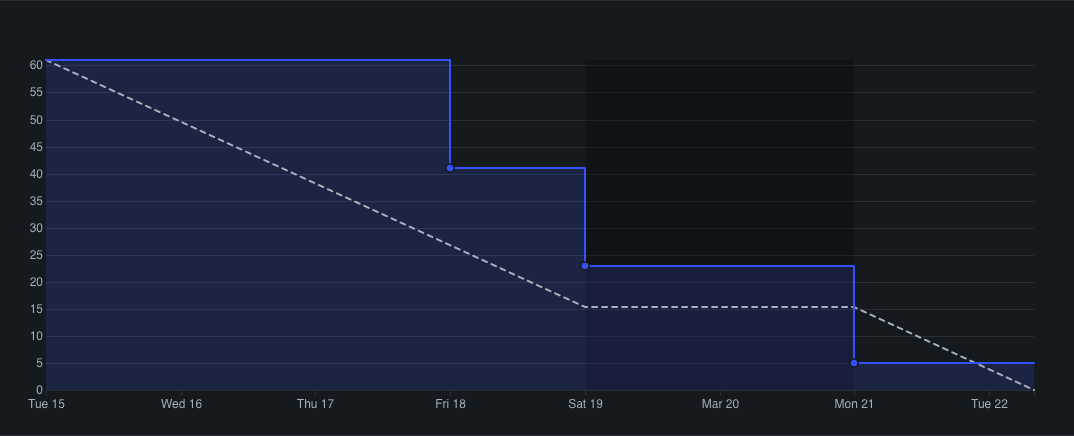
\includegraphics[width=\textwidth]{../img/anexos/sprints/BD-Sprint14}
\caption{\textit{Burndown Chart Sprint 14.}}\label{fig:BD-Sprint14}
\end{center}
\end{figure}
En este \textit{sprint} se han invertido cerca de 38h, el equipo de desarrollo cada vez se encuentra más cómodo trabajando en las diferentes tareas que se asignan, y aunque el número de puntos de historia es relativamente elevado, 60, esto es debido al histórico de dificultad de programar determinados algoritmos. 

\item \textbf{\textit{Sprint review meeting}}\\
Junto con lo expuesto anteriormente, se ha comprobado en este \textit{sprint} la implementación de los algoritmos basados en picos de densidad, con la corazonada de que no habría algún fallo en su implementación. Para sorpresa del equipo de desarrollo no han sido necesarios cambios a mayores de un par de <<fallos de dedo>> a la hora de programarlos, lo cual ha permitido una mayor agilidad a la hora de trabajar y reducir el número de horas invertidas.
\end{itemize}

\subsubsection{\textit{Sprint} 15: Robbie}
\begin{itemize}
\item \textbf{\textit{Planning meeting}}\\
Objetivos del decimoquinto \textit{sprint}:
\begin{enumerate}
\item Toma de decisión del formato del diagrama de secuencia <<Nuevo Experimento>>.
\item Introducir en Trabajos Relacionados, una disyunción entre \texttt{UBUMLaaS} y los el aprendizaje semi-supervisado seguro.
\item Comenzar con la primera etapa de experimentación <<seria>> que se va a realizar.
\item Segundo
\end{enumerate}

\item \textbf{Marcas temporales}\\
Este \textit{sprint} se desarrolla entre el 22/03/2022 y el 29/03/2022.

\item \textbf{\textit{Burndown chart}}\\
\begin{figure}
\begin{center}
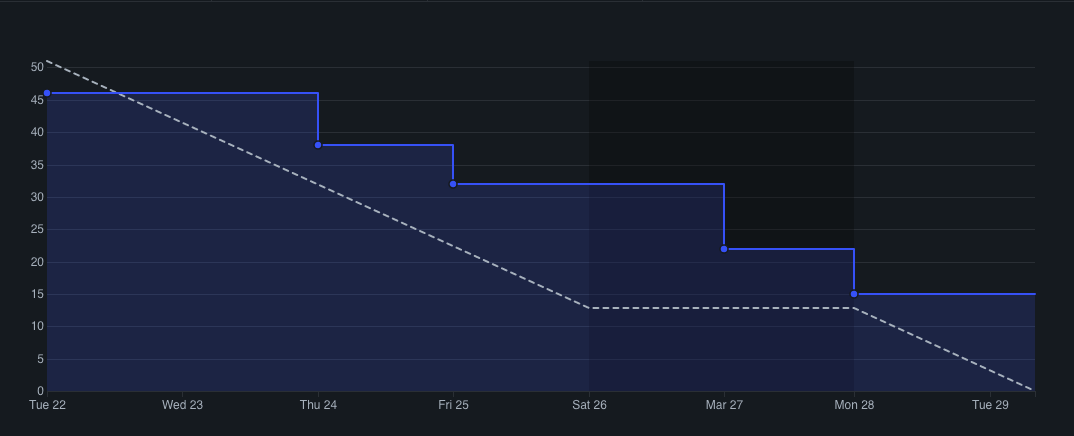
\includegraphics[width=\textwidth]{../img/anexos/sprints/BD-Sprint15}
\caption{\textit{Burndown Chart Sprint 15.}}\label{fig:BD-Sprint15}
\end{center}
\end{figure}
Lo primero a destacar de este \textit{sprint} y tal cual lo refleja la Figura~\ref{fig:BD-Sprint15}, correspondiente al \textit{Burndown report}; no se han terminado todas las tareas a tiempo. Esto ha sido debido a que faltaba por cerrar un \textit{pull request} el cual estaba pasando una serie de tests.

El número total de puntos de historia asignados al \textit{sprint} ha sido de 45, y se han invertido aproximadamente 35 horas, en esta ocasión el trabajo ha ido acorde a los puntos de historia asignados.

\item \textbf{\textit{Sprint review meeting}}\\
Con la experimentación lanzada y pudiendo haberse hecho entera, únicamente un sexto de lo que se espera que sea al final, los resultados no parecen ser muy prometedores, pero aún es pronto para saber lo que finalmente va a ser.\\

Los diagramas de secuencia han llevado mucho más tiempo del inicialmente esperado, esto se debe a la poca experiencia realizando este tipo de actividades y que no son el principal atractivo, por lo que el trabajo en esas partes se ha visto ralentizado.

En general todas las tareas relacionadas con la memoria están requiriendo más tiempo del que \textit{a priori} parece que va a ser necesario. Pero para conseguir un producto de calidad, es lo que se debe hacer.

\end{itemize}

\subsubsection{\textit{Sprint} 16: Matt 16}
\begin{itemize}
\item \textbf{\textit{Planning meeting}}\\
Objetivos del dieciseisavo \textit{sprint}:
\begin{enumerate}
\item Mejora de la calidad del código de los algoritmos de la biblioteca \texttt{IS-SSL}.
\item Remates de los diagramas de secuencia.
\item Añadir \textit{Self-Training} basado en picos de densidad~\cite{WU2018180} a los Conceptos Teóricos.
\item Escribir el Manual del Programador.
\item Crear ficheros de configuración de entorno para \texttt{Conda} y \texttt{Pyenv}.
\end{enumerate}

\item \textbf{Marcas temporales}\\
Este \textit{sprint} se desarrolla entre el 29/03/2022 y el 08/04/2022.

\item \textbf{\textit{Burndown chart}}\\
\begin{figure}
\begin{center}
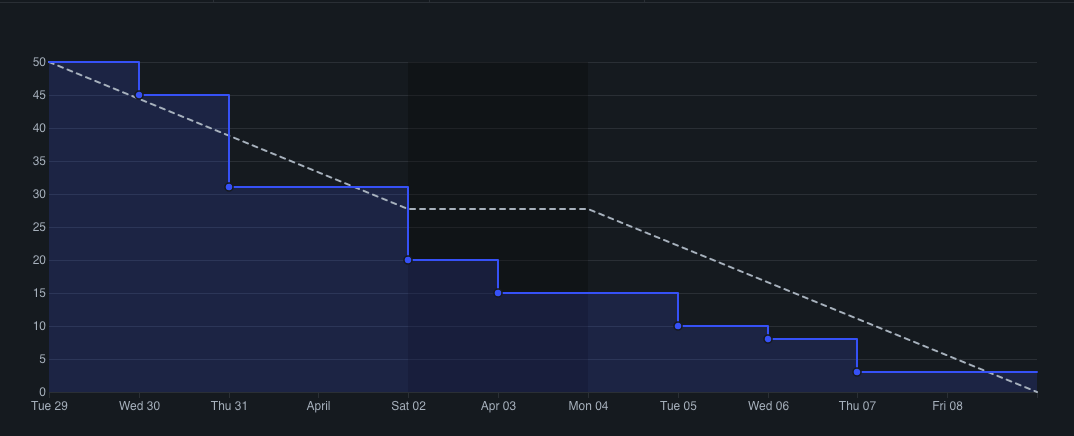
\includegraphics[width=\textwidth]{../img/anexos/sprints/BD-Sprint16}
\caption{\textit{Burndown Chart Sprint 16.}}\label{fig:BD-Sprint16}
\end{center}
\end{figure}
En este \textit{sprint} se ha trabajado principalmente en la memoria y en retoques de código, es por ello que se ha dado una cifra superior de puntos de historia de la media, y con lo visto en el \textit{sprint} anterior, estas tareas están comenzando a llevar más tiempo de que inicialmente se piensa. Se han invertido aproximadamente 37 horas. Los tiempos de trabajo empiezan a ser correctos de forma reiterada con lo planificado.

\item \textbf{\textit{Sprint review meeting}}\\
Con la experimentación a tres sextos realizada, todavía no se ha encontrado un nexo común que nos permita crear hipótesis, por lo que se aprovecharán las vacaciones de Semana Santa para dejar más experimentos en ejecución y rehacer las \textit{scripts} de análisis de resultados.

UBUMLaaS parece que está correcto en todas sus funcionalidades, por lo que ya se podría afirmar que la parte <<grande>> de modificación está terminada.

\end{itemize}

\subsubsection{\textit{Sprint} 17: Dae Han}
\begin{itemize}
\item \textbf{\textit{Planning meeting}}\\
Objetivos del decimoséptimo \textit{sprint}:
\begin{enumerate}
\item Modificar las tablas de versiones con una descripción.
\item Realizar una encuesta para utilizar agentes externos como \textit{beta testers} para UBUMLaaS.
\item Cambiar las \textit{Long Table} de los casos de uso por tablas normales de \LaTeX.
\item Escribir el anexo de la documentación técnica del programador.
\item Realizar los diagramas de relación.
\item Modificar los algoritmos de visualización de los resultados de la experimentación.
\end{enumerate}

\item \textbf{Marcas temporales}\\
Este \textit{sprint} se desarrolla entre el 08/04/2022 y 20/04/2022. Englobando las vacaciones de Semana Santa.

\item \textbf{\textit{Burndown chart}}\\
\begin{figure}
\begin{center}
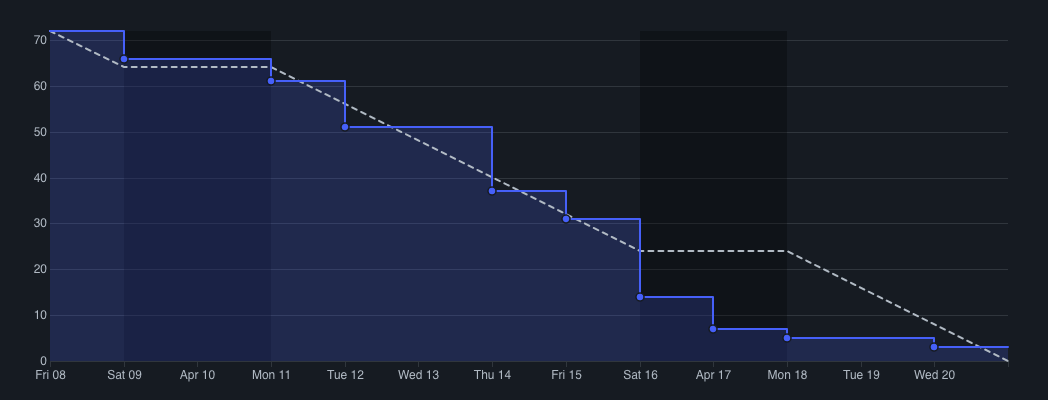
\includegraphics[width=\textwidth]{../img/anexos/sprints/BD-Sprint17}
\caption{\textit{Burndown Chart Sprint 17.}}\label{fig:BD-Sprint17}
\end{center}
\end{figure}
El trabajo a lo largo de este \textit{sprint} ha sido a ritmo constante, tal y como se aprecia en la Figura~\ref{fig:BD-Sprint17}, se aprecia como el número de puntos de historia es elevado, esto se debe a que se realizan en total 26 \textit{issues}, del total de 27 planificadas. Son muchas tareas pequeñas que acaban elevando el número de puntos de historia empleados. En total se han invertido alrededor de 45 horas de trabajo a lo largo de todo el\textit{sprint}.

\item \textbf{\textit{Sprint review meeting}}\\
En este \textit{sprint} se sobre-predijo el número de puntos de historia necesarios para resolver un número determinado de \textit{bugs} en \texttt{UBUMLaaS}, resultando estos más sencillos de resolver que en lo que en un primer momento parecía. 

Una tarea que quedó por cubrir fue la escritura de las pruebas que se han realizado en los productos \textit{software} desarrollados, no dando tiempo a finalizarlo en tiempo y forma.

El \textit{sprint} ha estado muy enfocado en mejorar la calidad del código de las bibliotecas de \texttt{IS-SSL}, así como la escritura de la memoria y anexos.

\end{itemize}

\subsubsection{\textit{Sprint} 18: Desforges}
\begin{itemize}
\item \textbf{\textit{Planning meeting}}\\
Objetivos del decimoctavo \textit{sprint}:
\begin{enumerate}
\item Por solapamiento con la asignatura de Minería de Datos, se va a introducir el algoritmo \texttt{RESSEL}~\cite{de2021reliable}.
\item Finalizar el anexo <<Especificación de Diseño>>.
\item Finalizar el anexo <<Documentación de usuario>>.
\item Realización del estudio de la viabilidad legal y económica del proyecto.
\item Actualizar la tabla de \emph{Experiments} en la base de datos de \texttt{UBUMLaaS} para que los algoritmos de \texttt{Scikit-Learn} sean compatibles con la versión 0.24.
\end{enumerate}

\item \textbf{Marcas temporales}\\
Este \textit{sprint} se desarrolla entre el 20/04/2022 y 02/05/2022.

\item \textbf{\textit{Burndown chart}}\\
\begin{figure}
\begin{center}
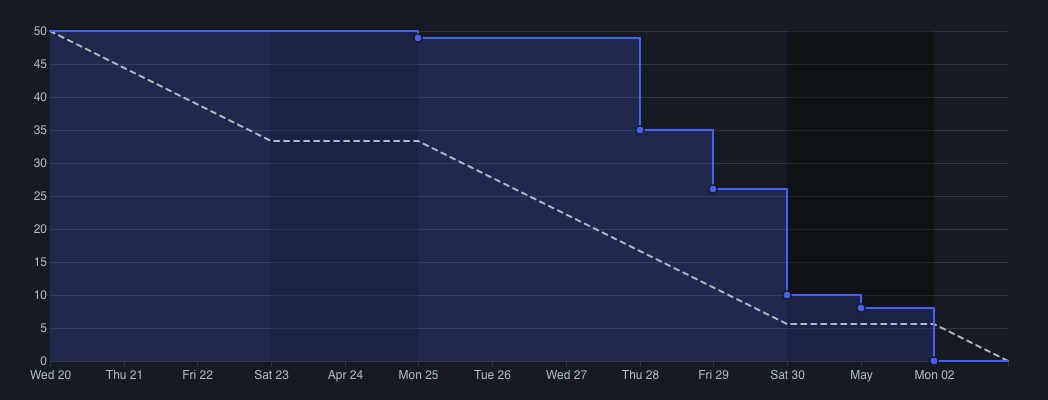
\includegraphics[width=\textwidth]{../img/anexos/sprints/BD-Sprint18}
\caption{\textit{Burndown Chart Sprint 18.}}\label{fig:BD-Sprint18}
\end{center}
\end{figure}
Tal y como se aprecia en la Figura~\ref{fig:BD-Sprint18}, en este \textit{sprint} el ritmo de trabajo no ha sido continuo, por motivos de índole personal la primera semana de trabajo no se pudieron cerrar prácticamente tareas, si bien si que se pudo avanzar en ellas permitiendo que cuando se dispuso de tiempo para trabajar a ritmo <<normal>> en ellas, éstas se cerraran con relativa sencillez.

El tiempo total invertido fue de 30 horas aproximadamente. Quedando cerrados 50 puntos de historia.

\item \textbf{\textit{Sprint review meeting}}\\
La calidad del producto que se está obteniendo está resultando satisfactoria para ambas partes, tanto el equipo de desarrollo como para el tutor del proyecto. 

Cabe destacar que el producto de documentación final (memoria y anexos) está empezando a ser relativamente grande, no siendo un mal indicador ya que a la fecha de finalización del \textit{sprint} ya se han realizado numerosas revisiones de la misma, pero ello no implica que no llame la atención.

Se detectó y solucionó un problema en los algoritmos de \textit{clustering} en \texttt{UBUMLaaS}, gracias a las pruebas realizadas por terceros sobre el proyecto. Además se actualizaron los algoritmos de \texttt{Scikit-Learn}, ya que su parametrización se había modificado y no permitía su ejecución.

\end{itemize}

\subsubsection{\textit{Sprint} 19: Rahoi}
\begin{itemize}
\item \textbf{\textit{Planning meeting}}\\
Objetivos del decimonoveno \textit{sprint}:
\begin{enumerate}
\item Mejora de la calidad del código de las bibliotecas \texttt{IS-SSL}, principalmente reducir la complejidad cognitiva de los algoritmos de aprendizaje semi-supervisado.
\item Mejora de la documentación del código de las librearías \texttt{IS-SSL}.
\item Solución de errores reportados por \texttt{SonarCloud} en \texttt{UBUMLaaS}.
\item Escritura de las pruebas de \texttt{IS-SSL} y \texttt{UBUMLaaS} en el anexo de <<Documentación técnica de programación>>.
\item Crear nuevas bases de datos <<limpias>> para desplegar en producción.
\item Embeber \texttt{UBUMLaaS} en un contenedor de \texttt{Docker} y dejarlo listo para su despliegue.
\item Crear gráficas de rankings para la experimentación.
\end{enumerate}

\item \textbf{Marcas temporales}\\
Este \textit{sprint} se desarrolla entre el 03/04/2022 y 10/05/2022.

\item \textbf{\textit{Burndown chart}}\\
\begin{figure}
\begin{center}
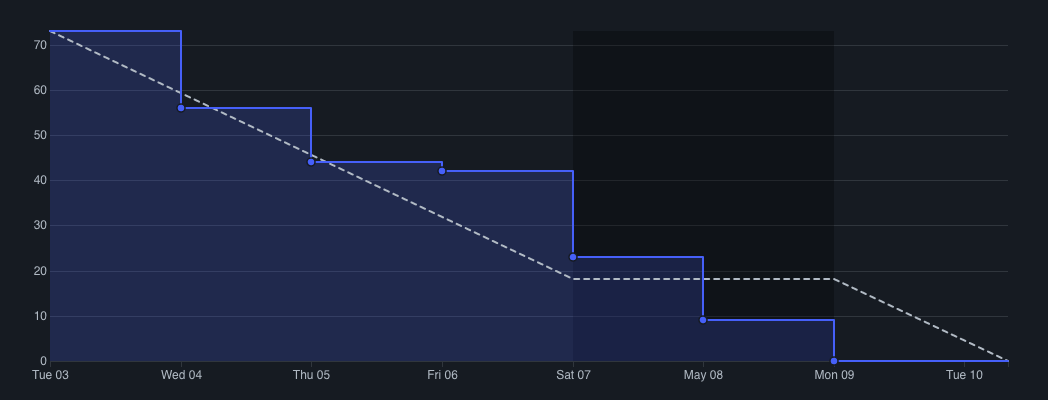
\includegraphics[width=\textwidth]{../img/anexos/sprints/BD-Sprint19}
\caption{\textit{Burndown Chart Sprint 19.}}\label{fig:BD-Sprint19}
\end{center}
\end{figure}
El trabajo en este \textit{sprint} ha ido al ritmo deseado, si bien en la Figura~\ref{fig:BD-Sprint19} se aprecia como el viernes 06 no se cerraron grandes tareas, el trabajo del sábado se vio afectado permitiendo cerrar más de las habituales. Ha sido un \textit{sprint} que ha requerido de bastantes horas <<extras>> de investigación y aprendizaje para poder cumplimentar todas las \textit{issues} correctamente.

Aproximadamente se han invertido cerca de 41 horas en el desarrollo del proyecto esta semana. Siendo resueltos 73 puntos de historia.

\item \textbf{\textit{Sprint review meeting}}\\
La calidad del producto está aumentando considerablemente, y a la vista de los resultados se aprecia la facilidad de mantenimiento. Gracias a las sucesivas iteraciones de mejora de la calidad, cada \textit{sprint} se puede mejorar y mantener el código con más facilidad, permitiendo <<hacer más en menos>>.

Un \textit{bug} que se detectó y paralizó el trabajo fue el descubrimiento de que \texttt{UBUMLaaS} había dejado de funcionar pero únicamente en sus capacidades de experimentación. Fue necesaria casi una jornada entera de trabajo para solucionar el problema. En el proceso de refactorizaciones se hicieron pequeños cambios en las declaraciones de las colas del sistema, anteriormente estando definidas por 4 \textit{workers}, y estos ya no son suficientes para el tamaño de la plataforma, cuando se aumentaron a 16, el problema desapareció.

Las gráficas de rankings no muestran una tendencia, será necesario calcular los rankings medios y realizar \textit{tests} estadísticos sobre estos para poder llegar a conclusiones.
\end{itemize}

\subsubsection{\textit{Sprint} 20: Klepto}
\begin{itemize}
\item \textbf{\textit{Planning meeting}}\\
Objetivos del vigésimo \textit{sprint}:
\begin{enumerate}
\item Crear \textit{tests} estadísticos para los rankings medios.
\item Introducir el trabajo de Triguero de aprendizaje semi-supervisado seguro~\cite{triguero2014characterization} en los <<Trabajos Relacionados>> de la memoria.
\item Revisar todas las tablas de la documentación y normalizar, así como hacerlas auto-contenidas si no lo son ya.
\item Añadir a la documentación las validaciones de los algoritmos implementados.
\item Crear y actualizar los repositorios de GitHub, en especial los README.
\item Escribir el <<Resumen>> e <<Introducción>> de la memoria.
\item Escribir una primera versión de las <<Conclusiones y Líneas futuras de trabajo>> de la memoria.
\end{enumerate}

\item \textbf{Marcas temporales}\\
Este \textit{sprint} se desarrolla entre el 10/04/2022 y 16/05/2022.

\item \textbf{\textit{Burndown chart}}\\

\item \textbf{\textit{Sprint review meeting}}\\

\end{itemize}

\newpage
\subsubsection{\textit{Sprint} n: Name}
\begin{itemize}
\item \textbf{\textit{Planning meeting}}\\
Objetivos del n \textit{sprint}:
\begin{enumerate}
\item Primero
\item Segundo
\end{enumerate}

\item \textbf{Marcas temporales}\\

\item \textbf{\textit{Burndown chart}}\\

\item \textbf{\textit{Sprint review meeting}}\\

\end{itemize}

\newpage
\section{Estudio de viabilidad}
En esta sección se va a desarrollar el estudio de la viabilidad del proyecto, permitiendo tener una visión global de los beneficios en contraposición al coste que supone el desarrollo del proyecto.

El desarrollo de cualquier producto \textit{software} conlleva una serie de riesgos, entre los que destacan la experiencia del equipo de desarrollo, el tamaño del proyecto, el tiempo del que se dispone para conseguirlo,\dots, influyendo todos ellos en el resultado final.
\subsection{Viabilidad económica}
Lo primero de todo que se va a calcular es la viabilidad económica del proyecto, reportando y analizando los costes/beneficios que habría supuesto el desarrollo del proyecto en el sector empresarial, en España\footnote{Se hace referencia al lugar de desarrollo puesto que se van a hacer referencias económicas en la moneda del país, así como uso de legislación vigente, la cuál varía en función del país en el que se encuentre asentada la empresa desarrolladora.}.

\subsubsection{Costes}
La realización de un proyecto de esta envergadura lleva asociados una serie de costes fijos y variables, a continuación se desglosan agrupados en \textit{hardware}, \textit{software}, personal, otros.

\textbf{Costes \textit{hardware}}

Para el desarrollo del proyecto es necesario más de un equipo \textit{hardware}, lo primero de todo es un equipo de tipo portátil. Se utilizará un MacBook Pro, con un procesador Inter Core i7 de 4 núcleos a 2.3~GHz, con 16~GB de memoria RAM, atendiendo a un precio de mercado de 2249~\officialeuro, se tiene en cuenta que la vida útil del equipo se encuentra en torno a los seis años, por lo que para los cálculos se usa la vida media del inmovilizado, es decir, 3 años. 

A su vez se necesita un servidor para desplegar la aplicación y trabajar sobre esta, ya que el despliegue local no se considera una forma de trabajo óptima. Es por ello que se hace uso de un equipo con un AMD FX(tm)-4130 Quad-Core a 4.5~GHz, con 64~GB de memoria RAM. El coste aproximado del equipo es de 1500~\officialeuro. La vida útil estimada es de seis ocho años, se utilizará igual que con el equipo portatil, su vida media de inmovilizado, 4 años.

La amortización para cada equipo es diferente, pero el tiempo de uso es el mismo, de noviembre de dos mil veintiuno a junio de dos mil veintidós, ambos incluidos, luego en total ocho meses. Se detallan todos los costes \textit{hardware} en la Tabla~\ref{tab:costes-hardware}.

\begin{table}[H]
\centering
\begin{tabular}{lrr}
	\toprule
	\textbf{Concepto} & \textbf{Coste (\officialeuro)} & \textbf{Coste Amortizado (\officialeuro)}\\
	\midrule
	Macbook Pro & 2.249 & 499,78\\
	Servidor & 1.500 & 250 \\
	\midrule
	\textbf{Total} & 3.049 & 749,78 \\
	\bottomrule
\end{tabular}
\caption{Costes de \emph{hardware}.}\label{tab:costes-hardware}
\end{table}

\textbf{Costes \textit{software}}

Para el desarrollo del proyecto y uso del \textit{software} necesario, es necesaria la adquisición de una serie de licencias, todas ellas se encuentran detalladas con su amortización en la Tabla~\ref{tab:costes-software}. Todas las licencias tienen un periodo de validez de un año.

\begin{table}[H]
\centering
\begin{tabular}{lrr}
	\toprule
	\textbf{Concepto} & \textbf{Coste (\officialeuro)} & \textbf{Coste Amortizado (\officialeuro)}\\
	\midrule
	Codacy & 170,76 & 113,84\\
	FileZilla & 0 & 0 \\
	GitKraken & 59,4& 36,27 \\
	Codacy & 170,76 & 113,84 \\
	Linux Mint 20.3 & 0 & 0 \\
	MacOs Monterey & 0 & 0 \\
	PyCharm & 240,79 & 160,53 \\
	Selenium & 0 & 0 \\
	SonarCloud & 120 & 80 \\
	\TeX Maker & 0 & 0 \\
	Travis-CI & 719,86 & 479,81 \\
	Visual Paradigm & 93,89 & 62,59 \\
	Visual Studio Code & 0 & 0~\\
	\midrule
	\textbf{Total} & 1.399,70 & 933,13 \\
	\bottomrule
\end{tabular}
\caption{Costes de \emph{software}.}\label{tab:costes-software}
\end{table}

\textbf{Coste de personal}
El desarrollo del proyecto ha sido llevado a cabo por un desarrollador y el tutor del proyecto.
\begin{itemize}
\item El salario del desarrollador se calcula según~\cite{SalarioJunior}, siendo el salario medio anal del 20.123~\officialeuro{} brutos al año.
\item El salario del tutor se calcula según~\cite{SalarioInvestigador}, siendo el salario medio anual de 22.784~\officialeuro{} brutos al año. Con una carga de trabajo de dos horas semanales.
\end{itemize}

La duración total del proyecto es de 31 semanas, por lo tanto, el tutor trabajará un total de 62 horas. Frente a las XXX del desarrollador.

El IRPF es del XX\% y la retribución a la Seguridad Social, calculada tal cual se plantea en~\cite{ss_cotizacion} por el Ministerio de Inclusión, Seguridad Social y Migraciones; se contribuye con un 31,40\% en total. Estando dividido en:
\begin{itemize}
\tightlist
\item 23,60\% de contingencias comunes~\cite{BOEPCM2442022}.
\item 5,50\% por desempleo de tipo general~\cite{BOEPCM2442022}.
\item 0,20\% destinado al Fondo de Garantía Salarial~\cite{BOEPCM2442022}.
\item 0,60\% de formación profesional~\cite{BOEPCM2442022}.
\item 1,50\% de tipo de cotización por accidentes de trabajo y enfermedades profesionales~\cite{BOEENFERMEDADES}.
\end{itemize}

\begin{table}[H]
\centering
\begin{tabular}{lrr}
	\toprule
	\textbf{Concepto} & \textbf{Desarrollador (\officialeuro)} & \textbf{Tutor (\officialeuro)}\\
	\midrule
	Salario total neto & XX & XX \\
	Retención IRPF & XX & XX \\
	Seguridad Social & XX & XX \\
	\midrule
	\textbf{Total salario bruto} & XX & XX \\
	\bottomrule
\end{tabular}
\caption{Costes de personal.}\label{tab:costes-personal}
\end{table}

En la Tabla~\ref{tab:costes-personal} se desglosan punto por punto los costes de personal, resultando en:
\[ XX\text{\officialeuro/desarrollador} + XX\text{\officialeuro/tutor} = XX\text{\officialeuro}\]

Siendo el coste total en personal de XX~\officialeuro.

\textbf{Otros costes}

Costes no agrupables en los anteriores apartados pero a tener en cuenta, Tabla~\ref{tab:costes-otros}.

\begin{table}[H]
\centering
\begin{tabular}{lr}
	\toprule
	\textbf{Concepto (\officialeuro)} & \textbf{Coste (\officialeuro)} \\
	\midrule
	Dominio despliegue & 32 \\
	Logos & 45 \\
	Memoria impresa & 250 \\
	Alquiler oficina & 1600 \\
	Internet & 136\\
	Electricidad & 140 \\
	Agua & 51\\
	Calefacción & 230 \\
	\midrule
	\textbf{Total} & 2484 \\
	\bottomrule
\end{tabular}
\caption{Otros costes.}\label{tab:costes-otros}
\end{table}

\textbf{Total de  costes}

En la Tabla~\ref{tab:costes-totales} se puede ver un resumen de todos los costes comentados. Dejando el coste base total del proyecto en XX~\officialeuro.

\begin{table}[H]
\centering
\begin{tabular}{lr}
	\toprule
	\textbf{Categoría (\officialeuro)} & \textbf{Coste (\officialeuro)} \\
	\midrule
	\textit{Hardware} & 3.049 \\
	\textit{Software} & 1.399,70 \\
	Personal & XX \\
	Otros & 2484 \\
	\midrule
	\textbf{Total} & 6.932,7+XX \\
	\bottomrule
\end{tabular}
\caption{Costes totales.}\label{tab:costes-totales}
\end{table}


\textbf{Beneficios}
El proyecto está compuesto de dos partes, las cuáles se pueden comercializar de forma independiente.
\begin{itemize}
\item \textbf{IS-SSL.} Las bibliotecas de algoritmos son distribuidas de forma pública, gratuita y sin publicidad, con el fin de aportar un <<granito de arena>> a la investigación en aprendizaje semi-supervisado y selección de instancias.
\item \textbf{UBUMLaaS.} En el diseño existente no está planteada su monetización. Si se quisiera obtener un rédito económico de este \texttt{MLaaS}, se podría fácilmente crear niveles de usuarios para acceso, número de experimentos máximos a lanzar. También se podría plantear como servicio de suscripción. En la Tabla~\ref{tab:opciones-beneficio} se plantean algunas posibilidades de comercialización con sus posibles respectivos costes para los usuarios, todas las licencias son anuales, en caso de un usuario quedarse sin tiempo podría comprar más horas de ejecución.
\end{itemize}

\begin{table}[H]
\centering
\begin{tabular}{lccrr}
	\toprule
	\textbf{Tipo}          &\textbf{Experimentos} & \textbf{Tiempo (h)} & \textbf{Precio (\officialeuro)} &  EUR/h\\
	\midrule
	\textit{Trial}        & 5 & 3 & 0 & X\\
	Estudiante   & 25 & 20 & 10 & X\\
	Investigador  & 120 & 250 & 40 & 0.4 \\
	Equipo  & 300 & 1000 & 150 & 0.4 \\
	Empresa & Ilimitados & 5000 & 2000 & 0.25 \\
	Otros & \multicolumn{3}{c}{Contactar con soporte para obtener presupuesto} \\
	\bottomrule
\end{tabular}
\caption{Opciones para obtener beneficio con UBUMLaaS.}\label{tab:opciones-beneficio}
\end{table}

Teniendo en cuenta los anteriores valores, y que la aplicación no tiene <<fronteras>> ya que el inglés es el idioma oficial de la investigación y la ciencia, se pueden alcanzar usuarios de todo el mundo. En la Tabla~\ref{tab:simulacion-clientes} se presenta un ejemplo real y viable de alcanzar la cuál permitiría recuperar la inversión del proyecto en el primer año.

\begin{table}[H]
\centering
\begin{tabular}{lcr}
	\toprule
	\textbf{Tipo}     & \textbf{Número de cuentas} & \textbf{Beneficios (\officialeuro)}\\
	\midrule
	\textit{Trial}        & Ilimitadas & 0 \\
	Estudiante   & 4 & 40 \\
	Investigador  & 15 & 600 \\
	Equipo  & 40 & 6.000 \\
	Empresa & 15 & 30.000 \\
	Otros & \multicolumn{2}{c}{No computado} \\
	\midrule
	\textbf{Total} &&36.640 \\
	\bottomrule
\end{tabular}
\caption{Simulación para recuperar la inversión con UBUMLaaS.}\label{tab:simulacion-clientes}
\end{table}

Debido a las funcionalidades ofrecidas y al precio competitivo de la plataforma, no sería difícil encontrar organizaciones que incorporen UBUMLaaS en su repertorio de herramientas, maximizando beneficios.

\textbf{Conclusiones}

Analizando los beneficios reportados en contraposción a los costes del desarrollo del proyecto, queda más que demostrada la viabilidad de desarrollo del proyecto. Se tiene en cuenta además que el proyecto una vez desarrollado no tiene necesidad de ser mantenido más allá de añadir nuevos algoritmos. Teniendo como costes fijos el mantenimiento de el(los) servidor(es) en donde esté desplegado.

\subsection{Viabilidad legal}

En esta sección principalmente se va a discutir el tema de licencias, ya que al ser un desarrollo \textit{software} es la temática más importante.

Según~\cite{softwareLicense}, una licencia de \textit{software} es un contrato entre la entidad que ha creado y suministrado una aplicación, el código fuente subyacente o un producto relacionado con el mismo, y su usuario final.  La licencia es un documento, habitualmente de texto, diseñado para proteger la propiedad intelectual del desarrollador del \textit{software} y para limitar cualquier reclamación contra él que pueda surgir de su uso.

Una licencia proporciona, además, definiciones legalmente vinculantes para la distribución y el uso del \textit{software}. Los derechos del usuario final, como la instalación,  las garantías y las responsabilidades, también se encuentran detallados en la licencia.


\subsubsection{\textit{Software}}
La licencia más importante es aquella bajo la cual se encuentra el \textit{software} desarrollado por el producto,  permitiendo el uso (sobretodo comercial y de distribución que se le puede dar). La principal limitación que se debe tener en cuenta es el orden jerárquico de licencias que se debe respetar. El proyecto utiliza una serie de dependencias externas, las cuáles poseen sus propias licencias, nunca pudiendo encontrarse bajo una licencia más permisiva.

A continuación se exponen las licencias de las dependencias utilizadas tanto por UBUMLaaS, Tabla~\ref{tab:dependencias-ubumlaas}, como por IS-SSL, Tabla~\ref{tab:dependencias-is-ssl}. La descripción de cada una se encuentra en las Tablas~\ref{tab:bibliotecas-python-ubumlaas}~y~\ref{tab:bibliotecas-python-is-ssl}, respectivamente.

\begin{table}[]
\centering
\begin{tabular}{lcl}
	\toprule
	\textbf{Dependencia} & \textbf{Versión} & \textbf{Licencia}\\
	\midrule
	\rowcolor[HTML]{EFEFEF} 
	\texttt{email-validator} & 1.1.1 & CC0 1.0 Universal\\
	\texttt{flask} & 1.1.1 & BSD 3 Clause\\ \rowcolor[HTML]{EFEFEF}
	\texttt{flask-login} & 0.4.1 & MIT\\
	\texttt{flask-mail} & 0.9.1 & BSD\\ \rowcolor[HTML]{EFEFEF}
	\texttt{flask-migrate} & 2.5.2 & MIT\\
	\texttt{flask-redis} & 0.4.0 & Blue Oak\\ \rowcolor[HTML]{EFEFEF}
	\texttt{flask-sqlalchemy} & 2.4.0 & BSD 3 Clause\\
	\texttt{flask-wtf} & 0.14.2 & BSD 3 Clause\\ \rowcolor[HTML]{EFEFEF}
	\texttt{future} & 0.16.0 & MIT\\ 
	\texttt{geopy} & 2.2.0 & MIT\\ \rowcolor[HTML]{EFEFEF}
	\texttt{glances} & 3.2.4.2 & GNU LGPLv3\\ 
	\texttt{imbalanced-learn} & 0.5.0 & MIT\\ \rowcolor[HTML]{EFEFEF}
	\texttt{itsdangerous} & 1.1.0 & BSD 3 Clause\\
	\texttt{liac-arff} & 2.2.1 & MIT \\ \rowcolor[HTML]{EFEFEF}
	\texttt{numpy} & 1.22.3 &BSD\\
	\texttt{pandas} & 0.25.1 & BSD 3 Clause\\ \rowcolor[HTML]{EFEFEF}
	\texttt{psutil} & 5.9.0 & BSD\\
	\texttt{pycountry} & 22.3.5 & GNU LGPLv2\\ \rowcolor[HTML]{EFEFEF}
	\texttt{pytest} & 5.2.1 & MIT\\
	\texttt{python-weka-wrapper3} & 0.1.7 & GNU GPLv3\\ \rowcolor[HTML]{EFEFEF}
	\texttt{requests} & 2.22.0 & Apache 2.0\\
	\texttt{rq} & 1.1.0 & BSD \\ \rowcolor[HTML]{EFEFEF}
	\texttt{scikit-learn} & 0.24 & BSD\\ 
	\texttt{selenium} & 3.141.0 & Apache 2.0\\ \rowcolor[HTML]{EFEFEF}
	\texttt{urllib3} & 1.25.6 & MIT\\
	\texttt{werkzeug} & 0.15.6 & BSD 3 Clause\\ \rowcolor[HTML]{EFEFEF}
	\texttt{whichcraft} & 0.4.1 & BSD \\
	\bottomrule
\end{tabular}
\caption{Bibliotecas utilizadas y sus versiones.}\label{tab:dependencias-ubumlaas}
\end{table}

\begin{table}[]
\centering
\begin{tabular}{lcl}
	\toprule
	\textbf{Biblioteca} & \textbf{Versión} & \textbf{Licencia}\\ \rowcolor[HTML]{EFEFEF} 
	\midrule
	\rowcolor[HTML]{EFEFEF} 
	\textbf{\texttt{numpy}}    & 1.20.3 &  BSD \\ \rowcolor[HTML]{EFEFEF} 
	\textbf{\texttt{pandas}}    & 1.3.4  & BSD 3 Clause  \\  
	\textbf{\texttt{scikit-learn}}    & 0.24.2 & BSD  \\ \rowcolor[HTML]{EFEFEF} 
	\textbf{\texttt{scipy}}    & 1.7.1  & BSD   \\ 
	\bottomrule
\end{tabular}
\caption{Bibliotecas utilizadas y sus versiones.}\label{tab:dependencias-is-ssl}
\end{table}

Como se aprecia en las Tablas~\ref{tab:dependencias-ubumlaas}~y~\ref{tab:dependencias-ubumlaas}, cada proyecto de manera individual va a estar sujeto a diferentes restricciones en cuanto a licencias se refiere, siendo más laxo en IS-SSL y mucho más restrictivo en UBUMLaaS. Para la comparación de licencias se utiliza JLA,~\cite{JLA}, \textit{joinup Licensing Assisntant}.

\imagenFlotante{../img/anexos/plan/Licencias}{Orden de permisividad/restricción de licencias.}{licencias}

En la Figura~\ref{fig:licencias} se detalla una comparación de las diferentes licencias de las dependencias de cada parte del proyecto, estando más a la derecha aquella con mayor restricciones, y a la izquierda la más permisivas. El \textit{software} debe estar licenciado como mínimo, con la más restrictiva.

\begin{itemize}
\item \textbf{UBUMLaaS.} Estará licenciado bajo GNU v3.  Figura~\ref{fig:licencia-ubumlaas}. 

Siendo una licencia perfecta para los objetivos de comercialización planteados. El \textit{software} se distribuye como \textit{open source} permitiendo que individuos lo usen de forma privada, pero en caso de que se quiera utilizar de cualquier manera de forma comercial deberá ser hecho \textit{open source}, permitiendo al equipo de desarrollo comprobar los cambios realizados, de forma que se puedan añadir al proyecto <<base>> u original.

\item \textbf{IS-SSL.} Estará licenciado bajo BSD Cláusula 3.  Figura~\ref{fig:licencia-is-ssl}.  El objetivo de las bibliotecas que conforman IS-SSL es que puedan ser ampliadas en cualquier momento por cualquier desarrollador, ya sea mediante \textit{pull requests} al proyecto o mediante sus propias implementaciones a través de \textit{forks}.  El objetivo del proyecto no es obtener un beneficio económico mediante licencias de uso, por lo tanto, BSD 3 se ajusta a las necesidades y requerimientos del proyecto.
\end{itemize}

\imagenFlotante{../img/anexos/plan/licencia-ubumlaas}{Licencia GNU v3 para UBUMLaaS.}{licencia-ubumlaas}
\imagenFlotante{../img/anexos/plan/licencia-is-ssl}{Licencia BSD 3 Clause para IS-SSL.}{licencia-is-ssl}

\subsubsection{Documentación}
La documentación del proyecto también se encuentra licenciada. En este caso no tiene sentido utilizar licencias similares a las anteriores puesto que no es un desarrollo \textit{software}, siendo más comunes y correctas licencias de tipo \textit{Creative Commons}. Se debe tener en cuenta el mismo principio anterior, todo aquel material de terceros que haya sido utilizado para la composición de la documentación, estará sujeto a licencias, no pudiendo ser distribuido con una licencia más permisiva que la que originalmente su autor lo distribuyó. 

En la documentación únicamente se han utilizado imágenes de terceros (unas pocas), estado todas ellas licenciadas bajo dominio público (CC0~\cite{CC0}), permitiendo utilizar cualquier licencia superior de \textit{Creative Commons} para licenciar la documentación.

Se ha decidido utilizar como licencia: \textit{Creative Commons Attribution-NonCommercial-NoDerivatives 4.0 International} (CC BY-NC-ND 4.0)~\cite{CCBYNCND40}.  En la Tabla~\ref{tab:licencia-documentacion} se resume lo que establece, así como acciones permitidas y prohibidas.

\begin{table}[H]
\centering
\begin{tabular}{ll}
	\toprule
	\textbf{Libre de} & \textbf{Bajo los términos}\\
	\midrule
	\multirow{3}{*}{Compartir - Copiar y redistribuir}   &Atribución\\
	    & No Comercial   \\  
	   & Sin Derivadas  \\ 
	\bottomrule
\end{tabular}
\caption{Bibliotecas utilizadas y sus versiones.}\label{tab:licencia-documentacion}
\end{table}
